\UseRawInputEncoding
\documentclass[conference]{IEEEtran}
\IEEEoverridecommandlockouts


\usepackage[utf8]{inputenc}  
\usepackage[T1]{fontenc}     
\usepackage{textcomp}        
\usepackage{amsmath,amssymb,amsfonts}
\usepackage{siunitx}                
\DeclareSIUnit\dbi{dBi}
\usepackage{graphicx}           
\usepackage{float}                 
\usepackage{placeins}     
\usepackage{url}           
\usepackage{cite}             
\usepackage{booktabs}
\usepackage{caption}             
\captionsetup{labelfont=bf, textfont=normalfont} 
\usepackage{listings}                
\usepackage{listingsutf8}             
\usepackage{xcolor}               
\definecolor{codebg}{RGB}{248,248,248}
\definecolor{codeframe}{RGB}{220,220,220}
\definecolor{codekw}{RGB}{0,92,197}
\definecolor{codestr}{RGB}{163,21,21}
\definecolor{codecmt}{RGB}{0,128,0}
% Creación del estilo "bonito" para Python / bloques de código de antena
\lstdefinestyle{bonito}{
    language=Python,
    backgroundcolor=\color{codebg},
    basicstyle=\ttfamily\small,
    keywordstyle=\color{codekw}\bfseries,
    stringstyle=\color{codestr},
    commentstyle=\color{codecmt}\itshape,
    numberstyle=\tiny\color{gray},
    numbers=left,
    stepnumber=1,
    frame=single,
    rulecolor=\color{codeframe},
    frameround=tttt,
    framesep=6pt,
    tabsize=2,
    showstringspaces=false,
    breaklines=true,
    upquote=true,
    % Configuración para evitar desbordamientos a la izquierda
    xleftmargin=2em,
    framexleftmargin=2em,
    numbersep=8pt
}

\raggedbottom                
\usepackage{titlesec}
\titlespacing*{\section}{0pt}{1.2ex plus .3ex minus .2ex}{0.8ex}
\titlespacing*{\subsection}{0pt}{1.0ex plus .3ex minus .2ex}{0.6ex}
\titlespacing*{\subsubsection}{0pt}{0.8ex plus .2ex minus .2ex}{0.5ex}

\setlength{\parskip}{0pt}           

\usepackage{enumitem}
\setlist{nosep}                     

\setlength{\abovecaptionskip}{4pt}
\setlength{\belowcaptionskip}{0pt}
\setlength{\textfloatsep}{10pt plus 1pt minus 2pt}
\setlength{\floatsep}{8pt plus 1pt minus 2pt}
\setlength{\intextsep}{8pt plus 1pt minus 2pt}
\renewcommand{\topfraction}{0.9}
\renewcommand{\bottomfraction}{0.8}
\renewcommand{\textfraction}{0.1}
\renewcommand{\floatpagefraction}{0.8}
\usepackage[hidelinks]{hyperref}


\def\BibTeX{{\rm B\kern-.05em{\sc i\kern-.025em b}\kern-.08em
    T\kern-.1667em\lower.7ex\hbox{E}\kern-.125emX}}
\begin{document}
%%%%%%%%%%%%%%%%%%%%%%%%%%%%%%%%%%%%%%%%%%%%%%%%%%%%%%%%%%%%%%%%%%%%%%%%%%%
\title{Enlace BPSK de telemetría industrial bajo ruido impulsivo: diseño Tx--canal--Rx, receptor con filtro acoplado, implementación SDR y evaluación BER\\
\author{\IEEEauthorblockN{Julian Camilo Acevedo Salamanca}
\IEEEauthorblockA{\textit{Universidad Industrial de Santander} \\
Bucaramanga, Colombia \\
Email: julian2224735@correo.uis.edu.co}
\and
\IEEEauthorblockN{Luigy Andrey Amado Durán}
\IEEEauthorblockA{\textit{Universidad Industrial de Santander} \\
Bucaramanga, Colombia \\
Email: luigy2230397@correo.uis.edu.co}
\and
\IEEEauthorblockN{Juan Camilo Salazar Ariza}
\IEEEauthorblockA{\textit{Universidad Industrial de Santander} \\
Bucaramanga, Colombia \\
Email: juan2212263@correo.uis.edu.co}

}
}
%%%%%%%%%%%%%%%%%%%%%%%%%%%%%%%%%%%%%%%%%%%%%%%%%%%%%%%%%%%%%%%%%%%%%%%%%%%%

\maketitle

% El documento se maneja por medio de importaciones para cada segmento esto con el fin de matener una estructura y facilitar el trabajo conjunto 

\begin{abstract}
An industrial telemetry link was designed for a process plant where motors, contactors and variable-frequency drives produce short, high-amplitude impulsive disturbances. The baseband model uses BPSK at $R_s=32$~ksym/s ($R_b=32$~kb/s), 8 samples per symbol and root-raised-cosine (RRC) pulse shaping with $\beta=0.35$, over a channel with additive white Gaussian noise plus a controlled periodic impulse train. The receiver applies an RRC matched filter, samples once per symbol at the eye maximum (offset 0, total delay of 11 symbols) and takes a minimum-distance decision. At the decision instants the matched filter reduces a single-sample impulse to 10\,\% of its amplitude, so with the project noise level no bit errors occurred for impulse amplitudes up to 5, although the decision margin fell from 0.88 to 0.40. The impulses were clearly visible in the time domain and in the constellation but barely in the power spectral density, where they only raised the floor and added a 1~kHz line comb. With differential encoding, the flowgraph reached a BER of $10^{-3}$ at $E_b/N_0=7.3$~dB, in agreement with theory; impulses of amplitude 1 caused no measurable penalty, whereas impulses of amplitude 5 caused a 1.8~dB penalty and a slowly decaying curve, explained by the symbols adjacent to each impulse. The link was also configured for HackRF One and USRP radios, together with the BER instrumentation for the experimental comparison.
\end{abstract}

\begin{IEEEkeywords}
BPSK, ruido impulsivo, filtro acoplado, RRC, BER, SDR, telemetría industrial; BPSK, impulsive noise, matched filter, root-raised cosine, bit error rate, software-defined radio.
\end{IEEEkeywords}

{\raggedright
\textit{Repositorio:} \href{https://github.com/juliancamiloacevedosalamanca-ship-it/ComunicacionesII_Grupo01}{github.com/juliancamiloacevedosalamanca-ship-it/ComunicacionesII\_Grupo01}\par}



\section{Introduction}
En una planta de proceso, un nodo sensor envía variables de baja velocidad ---temperatura, vibración y estado de una máquina--- hacia una estación de supervisión. El entorno contiene motores, contactores, variadores de frecuencia y cargas inductivas cuya conmutación produce perturbaciones electromagnéticas muy breves y de gran amplitud. Las mediciones en interiores identifican a los equipos con interruptores electromecánicos y a los motores como fuentes dominantes de ruido impulsivo de banda ancha \cite{blackard1993}, y su estadística se aparta del modelo gaussiano \cite{middleton1977}. En entornos industriales reales, este tipo de interferencia afecta enlaces de paquetes cortos y motiva técnicas de mitigación específicas \cite{zhan2022}.

El problema técnico no es aumentar la tasa de datos, sino conservar una señal reconocible y recuperar los bits cuando aparecen estos eventos. El trabajo se desarrolló en cuatro fases: modelado del canal con una perturbación impulsiva controlada; diseño de un transmisor con conformación de pulso y de un receptor digital propio; preparación del enlace sobre radios definidos por software (SDR), y caracterización del desempeño mediante curvas BER frente a $E_b/N_0$.

La Sección~\ref{sec:objetivos} define objetivos y alcance; la Sección~\ref{sec:metodologia} presenta el modelo, el transmisor, el receptor, la implementación SDR y la instrumentación; la Sección~\ref{sec:resultados} reporta y analiza los resultados, y la Sección~\ref{sec:conclusiones} resume las conclusiones.

% INTRODUCCIÓN (Escritura en presente/pasado, sin futuro)
\section{Objetivos y alcance}
\label{sec:objetivos}

\textbf{Objetivo general:} diseñar, simular y preparar para hardware SDR un enlace digital BPSK de telemetría industrial, con un receptor propio capaz de recuperar la información bajo un modelo de ruido AWGN más ruido impulsivo, y evaluar su desempeño mediante curvas BER frente a $E_b/N_0$.
    
\textbf{Objetivos específicos:}
\begin{enumerate}
    \item Relacionar los requerimientos de la aplicación con $R_s$, $R_b$, SPS, la tasa de muestreo y el filtro RRC.
    \item Diseñar el receptor (filtro acoplado, observación del ojo, muestreo y decisión) y validarlo en condición ideal y con el modelo de canal del proyecto.
    \item Cuantificar el efecto del ruido impulsivo en tiempo, frecuencia, constelación y tasa de error de bit.
    \item Configurar la interfaz con HackRF One y USRP sin alterar los parámetros de diseño y preparar la medición BER experimental.
\end{enumerate}

\textbf{Alcance:} el canal se modela en banda base con AWGN de amplitud 0.10 y un tren periódico de impulsos reales de amplitud $A_{imp}\in\{0,\,0.3,\,0.6,\,1.0\}$, un impulso cada 256 muestras; para el análisis de robustez se extiende a $A_{imp}=5$. En simulación se asume temporización ideal; en hardware se incorporan recuperación de frecuencia, reloj y fase. Las mediciones con el radio físico se realizan en el laboratorio con los flujogramas descritos.



\section{Metodología}
\label{sec:metodologia}

\subsection{Escenario y requisitos}
La Fig.~\ref{fig:escenario} muestra el escenario: el transmisor está montado sobre una banda transportadora accionada por un motor, cerca del tablero de contactores y del variador, y el receptor se ubica en la sala de supervisión. Si cien sensores reportan muestras de 16~bits a 10~Hz, la carga útil es 16~kb/s; con cabeceras y verificación de errores, $R_b=32$~kb/s deja un margen de 2:1. Se conservaron $R_s=32$~ksym/s y SPS~$=8$ porque cubren ese requerimiento, mantienen continuidad con la ficha de decisión y producen una tasa de banda base ($256$~kS/s) que se adapta a las tasas de los SDR con relaciones racionales sencillas.

\begin{figure}[H]
    \centering
    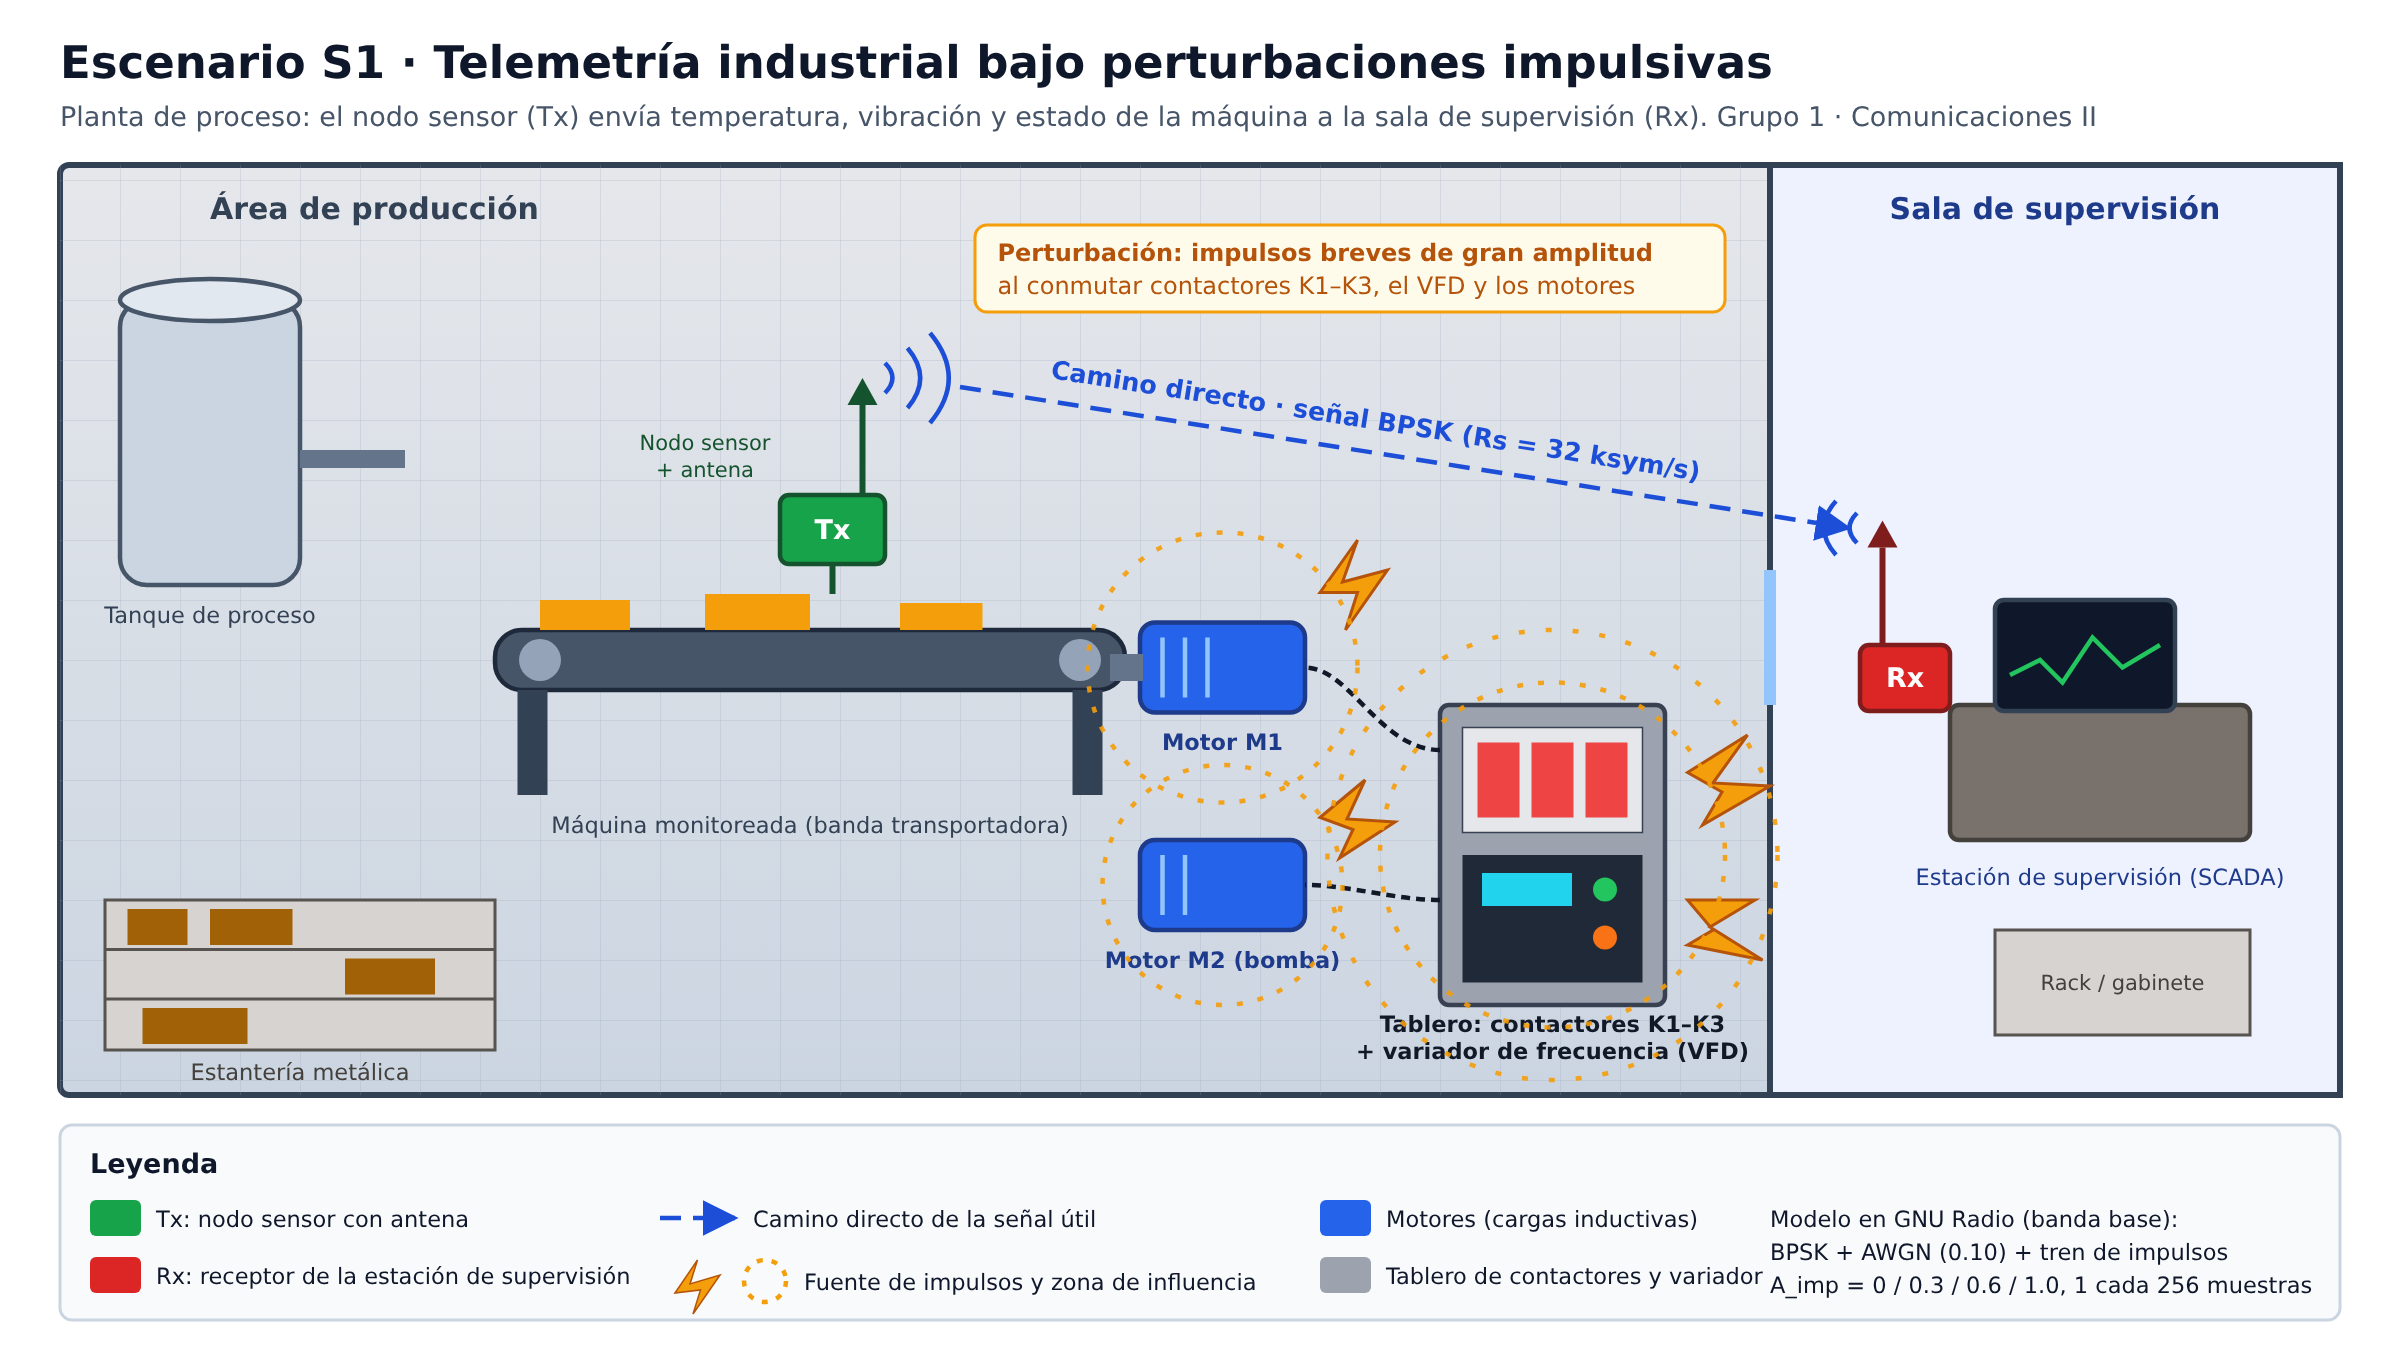
\includegraphics[width=\linewidth]{Figuras/escenario.png}
    \caption{Escenario contextual: nodo sensor (Tx), estación de supervisión (Rx) y fuentes de ruido impulsivo.}
    \label{fig:escenario}
\end{figure}

\subsection{Modelo del canal}
La señal recibida en banda base es
\begin{equation}
    r[n] = s[n] + w[n] + A_{imp}\sum_{k} \delta[n-255-256k],
    \label{eq:canal}
\end{equation}
donde $w[n]$ es AWGN complejo de potencia $0.10^2=0.01$. El tren de impulsos tiene potencia media $A_{imp}^2/256$, muy inferior a su potencia pico $A_{imp}^2$; este contraste explica gran parte de los resultados. Con la señal de potencia $\approx 1$, el AWGN equivale a $E_b/N_0\approx 29$~dB.

\subsection{Transmisor}
Se seleccionó BPSK ($M=2$, $k=\log_2 M=1$) porque, para una misma amplitud, ofrece la mayor distancia entre símbolos; se descartó OOK/ASK porque transporta la información en la amplitud, justamente lo que alteran los impulsos, y QPSK/16QAM porque aumentan $R_b$ sin necesidad y reducen la separación. Los bits provienen de una secuencia PRBS-15 conocida, se mapean como $0\rightarrow-1$, $1\rightarrow+1$ y se conforman con un filtro RRC de $\beta=0.35$ y longitud de 11 símbolos. La implementación genera $89$ coeficientes (número impar) con ganancia SPS, de modo que el nivel de cada símbolo es $\approx\pm1$. El ancho de banda ocupado es
\begin{equation}
    B \approx (1+\beta)R_s = 1.35\times 32~\text{kHz} = 43.2~\text{kHz},
    \label{eq:bw}
\end{equation}
frente a $\approx 64$~kHz entre primeros nulos del pulso rectangular usado en la fase de canal. La Tabla~\ref{tab:parametros} resume los parámetros.

\begin{table}[H]
    \centering
    \caption{Parámetros del enlace}
    \label{tab:parametros}
    \footnotesize
    \setlength{\tabcolsep}{4pt}
    \begin{tabular}{@{}lcc@{}}
        \toprule
        \textbf{Parámetro} & \textbf{Valor} & \textbf{Relación} \\
        \midrule
        Modulación & BPSK & $M=2$ \\
        Tasa de símbolos $R_s$ & 32 ksym/s & requisito \\
        Tasa de bits $R_b$ & 32 kb/s & $R_s\log_2 M$ \\
        Muestras por símbolo & 8 & -- \\
        Tasa de banda base & 256 kS/s & $R_s\cdot\text{SPS}$ \\
        Roll-off / span & 0.35 / 11 & -- \\
        Ancho de banda & 43.2 kHz & $(1+\beta)R_s$ \\
        AWGN del canal & 0.10 & $E_b/N_0\approx29$ dB \\
        Período de impulsos & 256 muestras & 1 ms \\
        \bottomrule
    \end{tabular}
\end{table}

\subsection{Receptor}
El receptor cumple cuatro funciones. \emph{Filtrado:} un filtro RRC acoplado con coeficientes $h_{rx}[n]=h[n]/\sum h^2$, de modo que la cascada Tx--Rx es un coseno alzado sin interferencia intersimbólica y el valor de decisión vale $\pm1$. \emph{Observación:} un diagrama de ojo a la salida del filtro acoplado. \emph{Muestreo:} cada filtro de 89 coeficientes introduce un retardo de 44 muestras; el retardo total es 88 muestras, exactamente 11 símbolos, por lo que se conserva una muestra de cada 8 con desfase 0, y la secuencia recuperada está retrasada 11 bits respecto a la transmitida. \emph{Decisión:} distancia mínima a los puntos $\pm1$, equivalente al umbral $I=0$.

El filtro acoplado también atenúa los impulsos: un impulso de una sola muestra aparece a la salida multiplicado por la forma del filtro, con un valor máximo
\begin{equation}
    \frac{\max_n h[n]}{\sum_n h^2[n]} = \frac{1.092}{7.94} = 0.137,
    \label{eq:atenuacion}
\end{equation}
de modo que un impulso de amplitud $A_{imp}$ desplaza la variable de decisión como máximo $0.137\,A_{imp}$.

\subsection{Implementación con SDR}
La Fig.~\ref{fig:sistema} muestra la arquitectura completa, implementada en un entorno de radio definida por software \cite{gnuradio,ortega2019}. Para hardware se conservan la modulación, $R_s$, SPS, $\beta$ y la decisión, y se agregan los parámetros propios del radio: frecuencia central $f_c=915$~MHz (banda ISM 902--928~MHz, sujeta a autorización del laboratorio), tasa del radio de 2~MS/s en HackRF One \cite{hackrf} y 1~MS/s en USRP \cite{uhd}, y remuestreo racional $256\,\text{k}\times125/16=2$~MS/s ($\times125/32$ para USRP), con la operación inversa en recepción. Los osciladores se sintonizan en $f_c\mp200$~kHz y la señal se desplaza digitalmente para alejarla de la componente de continua del conversor. Se eliminó el bloque de regulación de ritmo, porque el radio fija la tasa de muestras. Como los dos radios tienen osciladores independientes, el receptor de hardware agrega control automático de ganancia, un lazo de frecuencia de borde de banda, sincronización de reloj con banco polifásico de filtros RRC y un lazo de Costas de orden 2; para resolver la ambigüedad de fase de 180° se usa codificación diferencial.

\begin{figure*}[t]
    \centering
    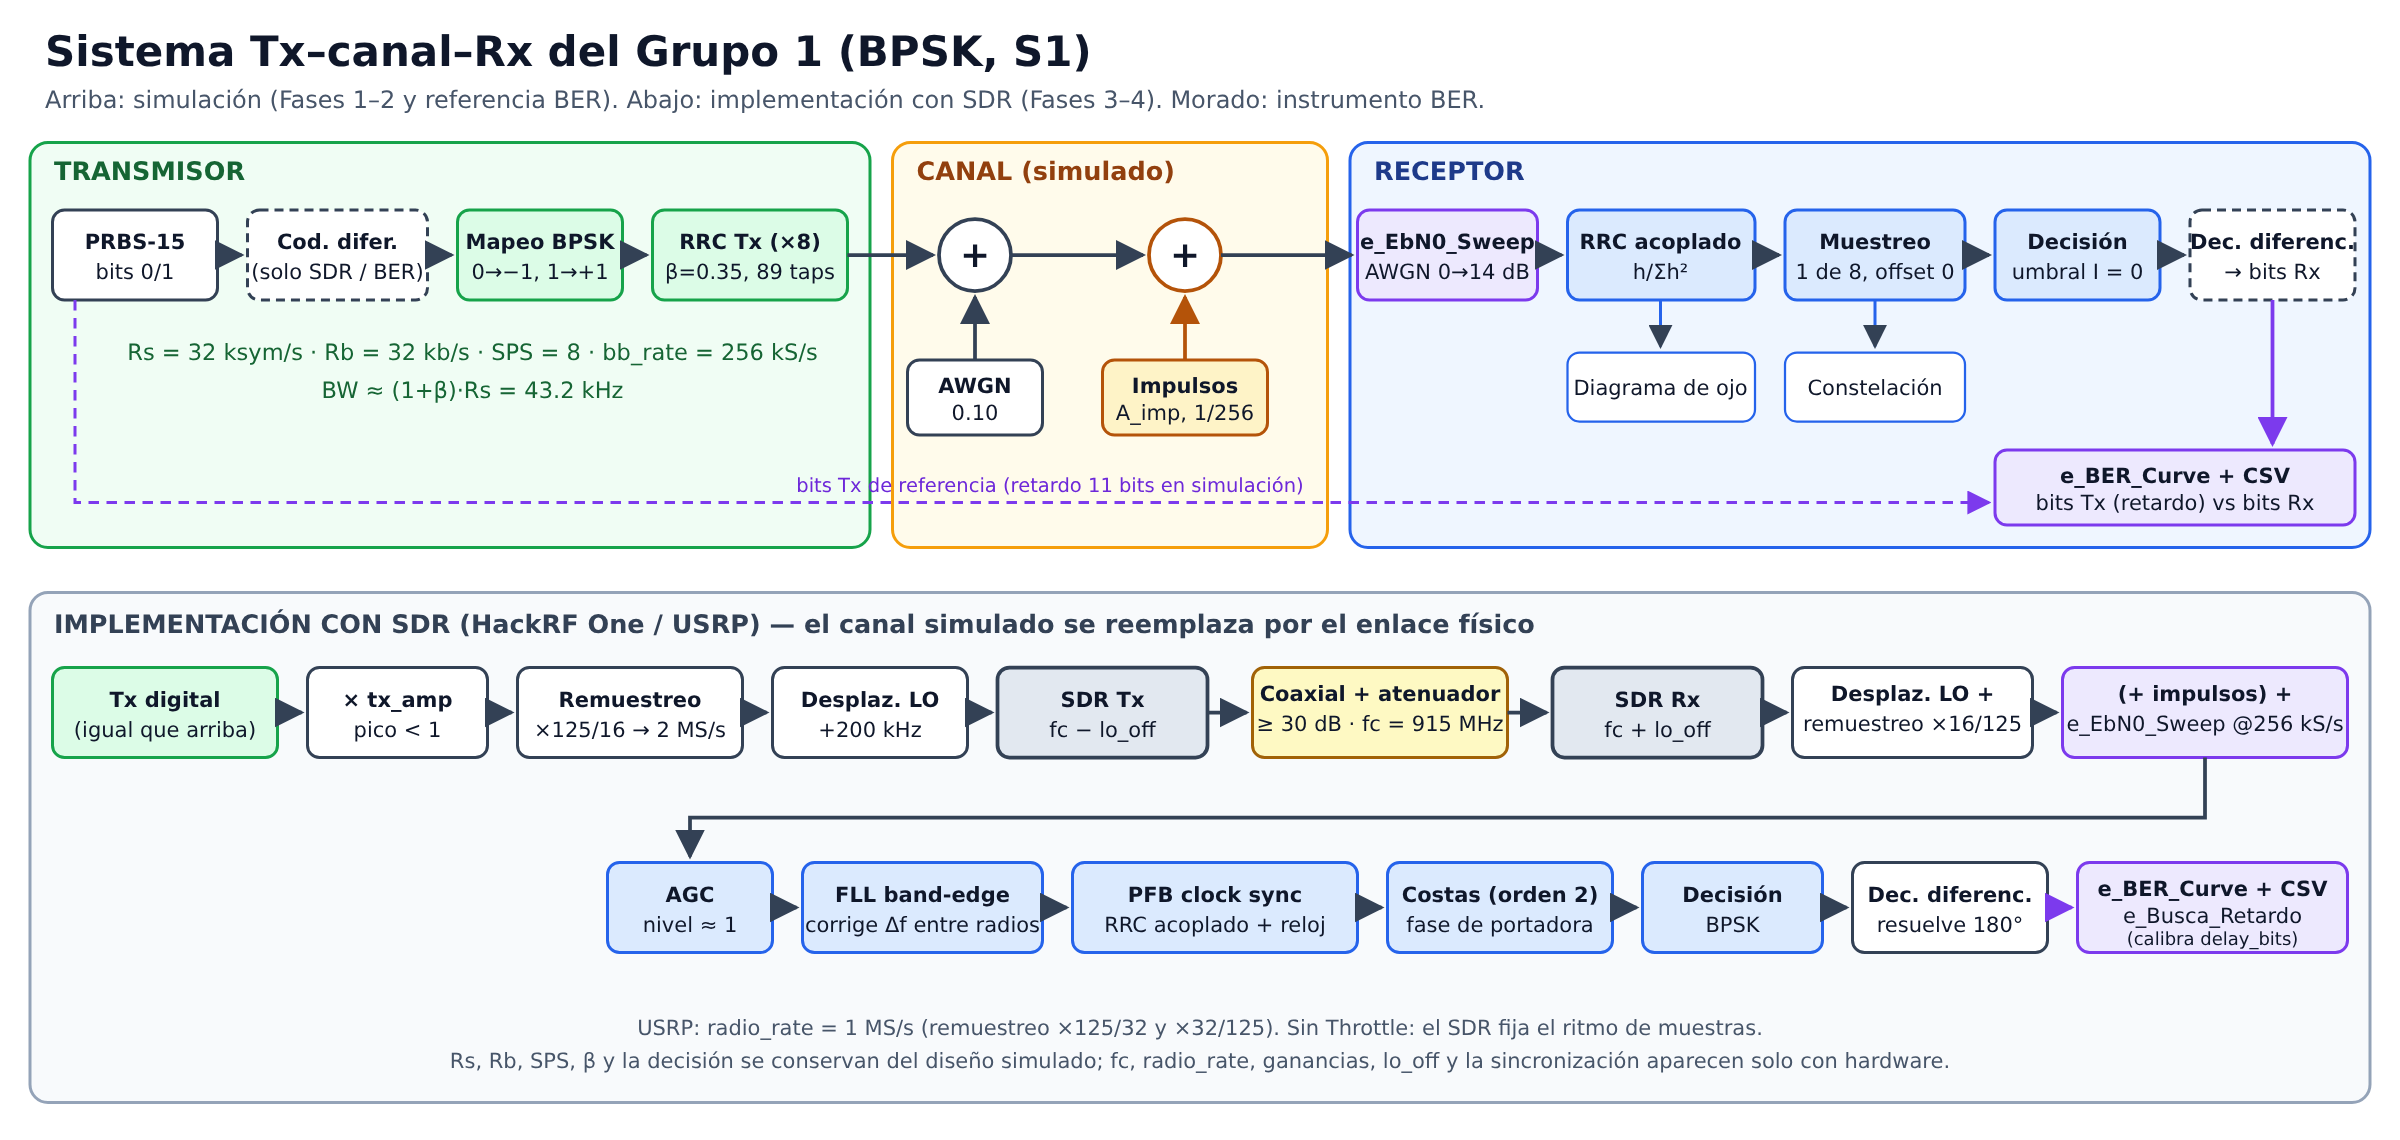
\includegraphics[width=0.92\textwidth]{Figuras/sistema_txrx.png}
    \caption{Arquitectura Tx--canal--Rx: simulación (arriba) e implementación con SDR (abajo), con el instrumento de medición BER.}
    \label{fig:sistema}
\end{figure*}

\subsection{Instrumentación BER}
Se integró el instrumento del curso: un bloque inserta AWGN controlado inmediatamente antes del receptor, con potencia
\begin{equation}
    P_n = \frac{P_s\,f_s}{R_b\,10^{(E_b/N_0)/10}},
    \label{eq:pn}
\end{equation}
y recorre $E_b/N_0$ de 0 a 14~dB en pasos de 1~dB, con $10^5$ bits por punto y $10^3$ bits de guarda; otro bloque compara los bits transmitidos (retrasados \texttt{delay\_bits}) con los recuperados y guarda la curva en un archivo CSV. Como referencia teórica se usa $P_b=Q\!\left(\sqrt{2E_b/N_0}\right)$ para BPSK y $P_b\approx2Q(1-Q)$ con codificación diferencial \cite{proakis2008}. Para calibrar \texttt{delay\_bits} en hardware se desarrolló un bloque que estima el retardo por correlación cruzada (Anexo~\ref{app:retardo}).
 
% MARCO TEÓRICO / METODOLOGÍA (Explicación de la teoría)}

\section{Resultados y discusión}
\label{sec:resultados}

Los resultados se presentan en el orden de las fases del proyecto: caracterización del canal (Fase~1), diseño y validación del sistema Tx--canal--Rx (Fase~2), configuración de la interfaz SDR (Fase~3) y medición de curvas BER (Fase~4). Todas las figuras de GNU Radio son capturas de los flujogramas del grupo en ejecución; las capturas completas de cada prueba están en el Anexo~\ref{app:capturas}.

\subsection{Fase 1: caracterización del canal con ruido impulsivo}
En la primera fase se partió del flujograma base del curso y se modificó para el escenario S1 (Anexo~\ref{app:fase1}): la tabla de símbolos pasó de OOK a BPSK $(-1,+1)$ y se agregó un tren de impulsos reales de amplitud $A_{imp}$, uno cada 256 muestras (1~ms), sumado a la salida del AWGN. En esta fase el pulso era rectangular de 8 muestras y no había receptor; se observaron la señal temporal, la constelación de las muestras y la PSD para la referencia y para las tres severidades de la Tabla~\ref{tab:fase1}, con $R_s$, SPS y $f_s$ fijos.

\begin{figure*}[t]
    \centering
    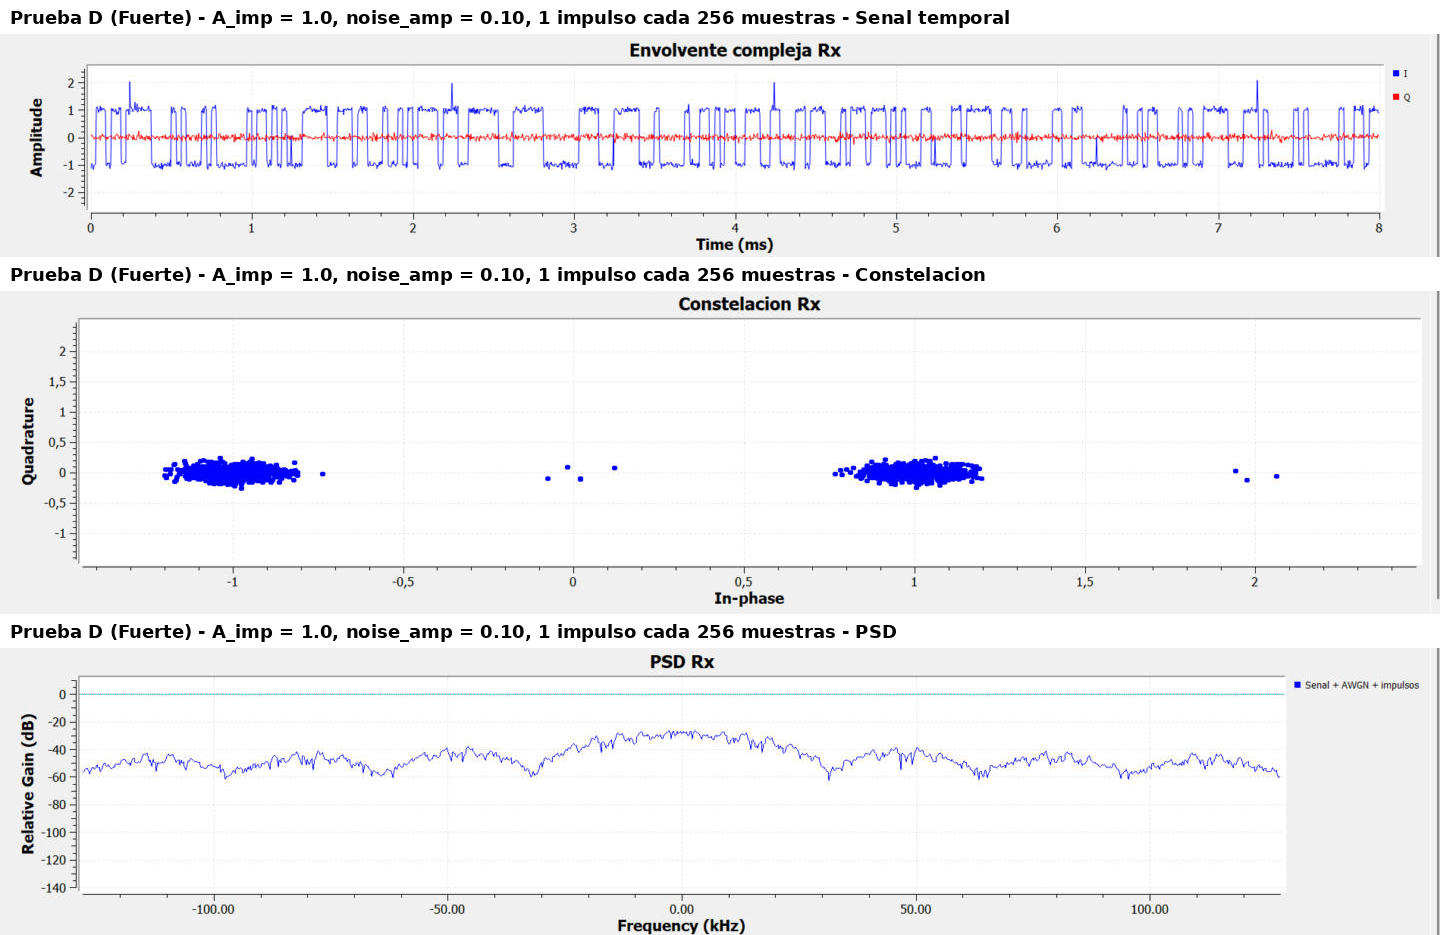
\includegraphics[width=0.82\textwidth]{Figuras/fase1_pruebaD.png}
    \caption{Fase~1, prueba D ($A_{imp}=1$, AWGN 0.10, pulso rectangular): envolvente compleja, constelación de las muestras y PSD a la salida del canal.}
    \label{fig:fase1}
\end{figure*}

\begin{table}[H]
    \centering
    \caption{Pruebas de la Fase 1 (pulso rectangular, sin receptor)}
    \label{tab:fase1}
    \footnotesize
    \setlength{\tabcolsep}{3pt}
    \begin{tabular}{@{}lcp{2.0cm}p{2.3cm}@{}}
        \toprule
        \textbf{Prueba} & $\mathbf{A_{imp}}$ & \textbf{Tiempo} & \textbf{Constelación} \\
        \midrule
        A (referencia) & 0.0 & niveles $\pm1$, sin picos & dos nubes en $\pm1$ \\
        B (suave) & 0.3 & picos de $\approx1.3$ cada 1 ms & puntos sueltos en $-0.7$ y $1.3$ \\
        C (media) & 0.6 & picos de $\approx1.6$ & puntos sueltos en $-0.4$ y $1.6$ \\
        D (fuerte) & 1.0 & picos de $\approx2$ & puntos sueltos en 0 y 2 \\
        \bottomrule
    \end{tabular}
\end{table}

La Fig.~\ref{fig:fase1} resume la prueba más severa. En el tiempo aparecen 8 picos en 8~ms, uno por milisegundo y solo en la componente I, porque el impulso es real. En la constelación, el AWGN abre cada símbolo en una nube, mientras que los impulsos producen unos pocos puntos aislados desplazados exactamente $+A_{imp}$ (una muestra de cada 256). La PSD conserva la forma $\mathrm{sinc}^2$ del pulso rectangular, con nulos en múltiplos de 32~kHz y unos 64~kHz entre primeros nulos, y casi no cambia entre pruebas: la potencia media del tren ($A_{imp}^2/256\le0.004$) es menor que la del AWGN (0.01). El hallazgo clave de esta fase es que, sin filtro acoplado, con $A_{imp}=1$ los puntos que venían del símbolo $-1$ caen en 0, justo en el umbral de decisión. Esto motivó dos decisiones de la Fase~2: conformar con RRC para reducir el ancho de banda y usar un filtro acoplado que reparta la energía del impulso antes de decidir.

\subsection{Fase 2: diseño y validación del sistema Tx--canal--Rx}
La Fig.~\ref{fig:flujograma} muestra el flujograma del enlace completo de la Fase~2. Las figuras de las secciones de espectro y receptor son capturas de ese flujograma en ejecución, con AWGN de amplitud 0.10 y la BER medida sobre una ventana de $10^5$ bits. Para los márgenes de decisión y como verificación de las curvas BER se usó además una simulación numérica que reproduce el flujograma bloque a bloque: los mismos 89 coeficientes RRC en Tx y Rx, el mismo retardo de 11 bits, la misma regla de decisión y la misma ley de inyección de ruido de la ecuación~\eqref{eq:pn}. Ambas coinciden: el flujograma midió BER $=0$ en las pruebas A a E y 0.2498 con 4 muestras de desfase, y la simulación dio 0 y 0.25.

Antes de las pruebas con perturbación, el receptor se validó en condición ideal, sin ruido ni impulsos (prueba 0, Anexo~\ref{app:capturas}). En ese caso la PSD del canal coincide con la del transmisor, la constelación recuperada se reduce a dos puntos exactos en $\pm1$ y la BER es cero: el filtro acoplado, el muestreo con desfase 0 y la referencia retrasada 11 bits funcionan sin errores antes de agregar el canal del proyecto.

\begin{figure*}[t]
    \centering
    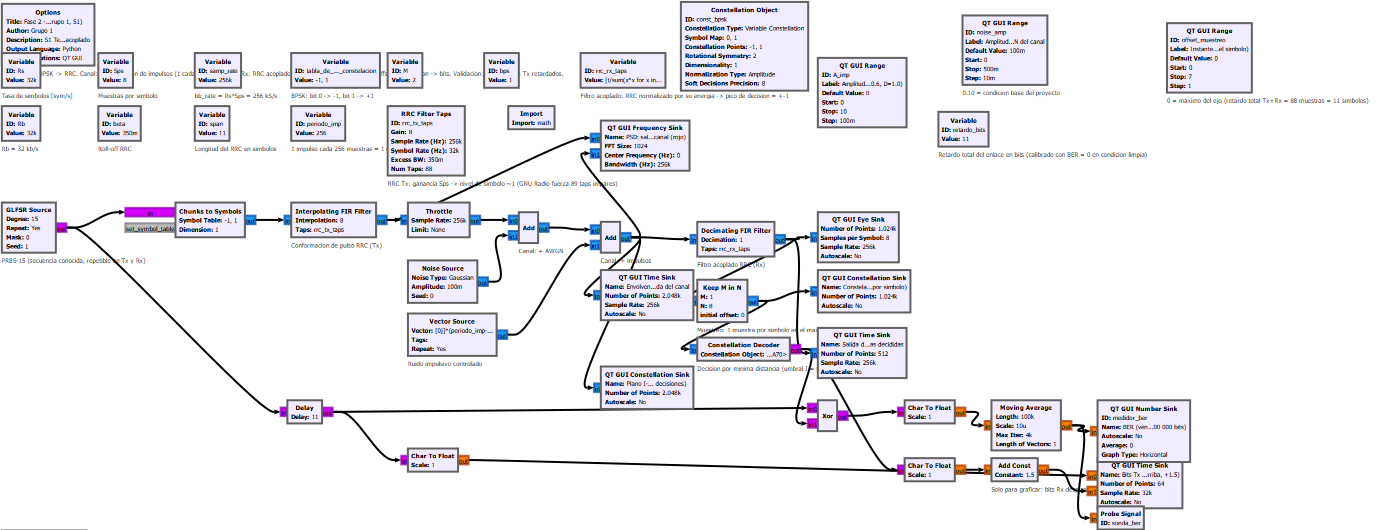
\includegraphics[width=0.95\textwidth]{Figuras/flujograma_fase2.png}
    \caption{Flujograma del enlace de la Fase~2: transmisor PRBS--BPSK--RRC, canal con AWGN y tren de impulsos, receptor con filtro acoplado, muestreo y decisión, y comparación de bits con la referencia retrasada 11 bits.}
    \label{fig:flujograma}
\end{figure*}

\subsubsection{Espectro y señal en el canal}
En la Fig.~\ref{fig:psd}, la señal a la salida del RRC del transmisor ocupa $\pm21.6$~kHz, como predice la ecuación~\eqref{eq:bw}, y fuera de esa banda sus lóbulos laterales caen más de 30~dB. Al agregar el canal, el AWGN fija un piso plano unos 30~dB por debajo de la banda de la señal. Con $A_{imp}=1$ el espectro casi no cambia respecto a la referencia: la potencia media del tren de impulsos es $1/256\approx0.004$, menos de la mitad de la del AWGN, y el piso sube apenas 1.5~dB (las capturas completas de todas las pruebas están en el Anexo~\ref{app:capturas}). Con $A_{imp}=5$ la potencia del tren es $25/256\approx0.098$, el piso sube unos 10~dB y aparece un peine de líneas separadas 1~kHz, que es la frecuencia de repetición de los impulsos (un impulso cada 256 muestras a 256~kS/s). La PSD, por ser un promedio, informa poco sobre el riesgo real: un evento de amplitud 5 en una sola muestra apenas se nota en ella.

\begin{figure*}[t]
    \centering
    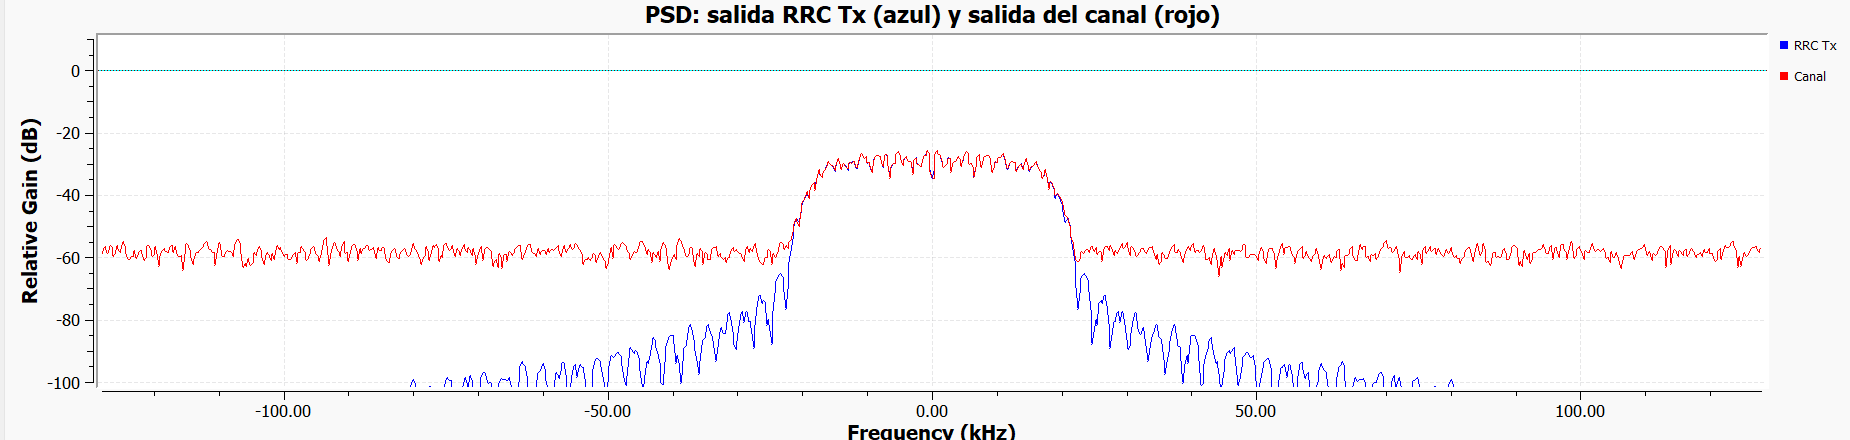
\includegraphics[width=0.49\textwidth]{Figuras/psd_A0.png}\hfill
    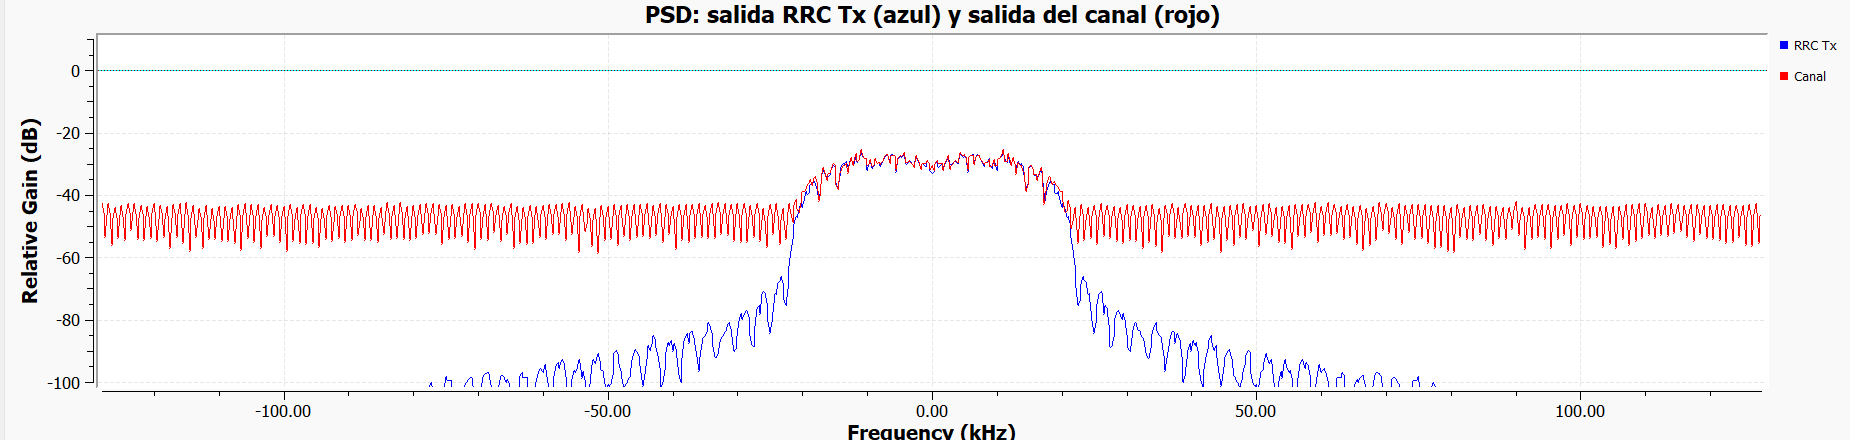
\includegraphics[width=0.49\textwidth]{Figuras/psd_A5.png}
    \caption{PSD a la salida del RRC del transmisor (azul) y a la salida del canal (rojo), con AWGN 0.10: prueba de referencia $A_{imp}=0$ (izquierda) y prueba de robustez $A_{imp}=5$ (derecha).}
    \label{fig:psd}
\end{figure*}

En el dominio del tiempo (Fig.~\ref{fig:tiempo}), en cambio, el impulso sí es visible: aparece solo en la componente I, porque es real, cada 1~ms. Su efecto depende del símbolo que coincide con él: sobre un nivel positivo produce un pico que supera 2, y sobre uno negativo reduce el nivel hacia cero.

\begin{figure}[H]
    \centering
    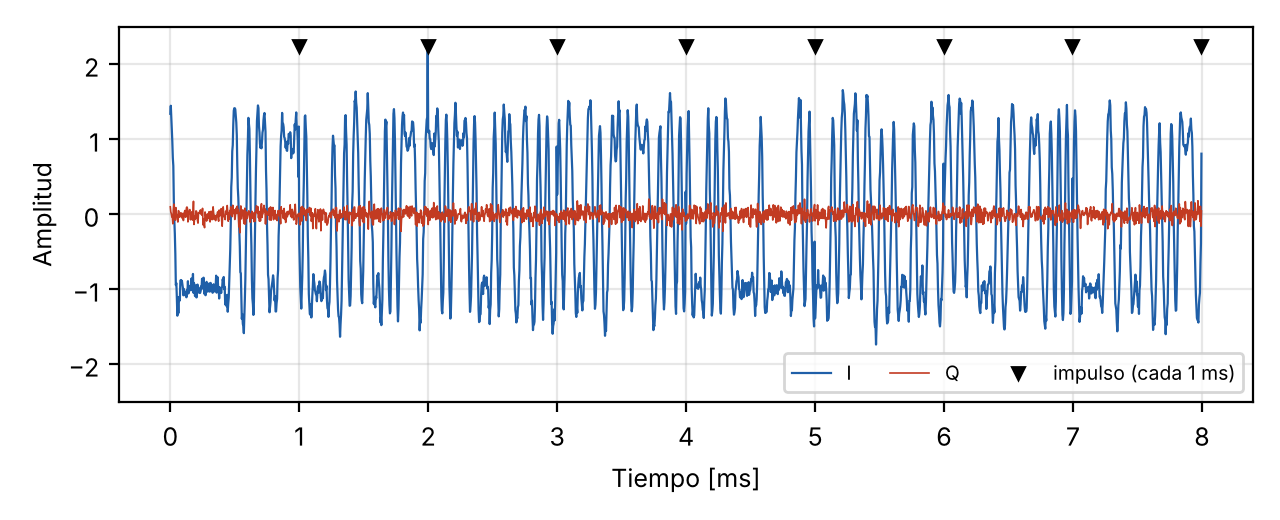
\includegraphics[width=\linewidth]{Figuras/tiempo_canal.png}
    \caption{Envolvente compleja a la salida del canal con $A_{imp}=1$ (8~ms; I en azul, Q en rojo). Los picos aislados de la componente I, uno por milisegundo, son los impulsos.}
    \label{fig:tiempo}
\end{figure}

\subsubsection{Receptor: ojo, constelación y bits}
La Fig.~\ref{fig:ojos} muestra el ojo a la salida del filtro acoplado. Con $A_{imp}=0$ las trayectorias convergen en $\pm1$ en los instantes de muestreo: la cascada RRC--RRC se comporta como un coseno alzado y no deja interferencia intersimbólica. Con $A_{imp}=0.6$ y $1.0$ el ojo es prácticamente el mismo. Solo con $A_{imp}=5$ aparecen trayectorias aisladas que se salen del haz, y aun así el ojo sigue abierto en el centro.

\begin{figure}[H]
    \centering
    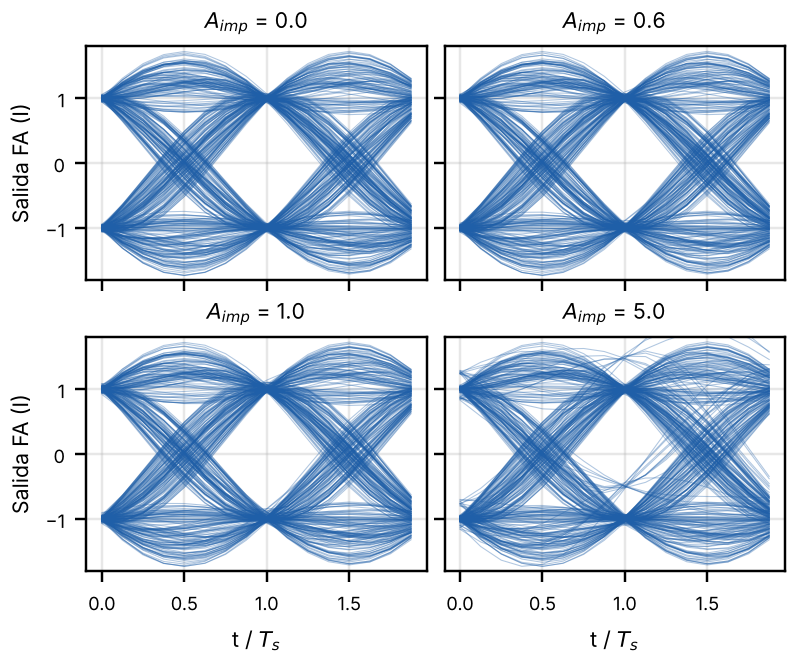
\includegraphics[width=\linewidth]{Figuras/ojos.png}
    \caption{Diagramas de ojo a la salida del filtro acoplado (componente I, dos símbolos).}
    \label{fig:ojos}
\end{figure}

La explicación está en el filtro acoplado. Un impulso de una muestra no se suma de forma directa a la variable de decisión: sale del filtro convertido en la forma del pulso, escalado por $1/\sum h^2$. Como el período de 256 muestras es múltiplo de SPS~$=8$, el impulso cae siempre en la misma fase dentro del símbolo, y en los instantes de muestreo su contribución máxima es $0.100\,A_{imp}$ (algo menor que la cota de 0.137 de la ecuación~\eqref{eq:atenuacion}, que corresponde al pico del pulso). Con $A_{imp}=1$ la muestra más afectada se corre $0.10$, frente a una distancia de 1 al umbral. Por eso la constelación recuperada (Fig.~\ref{fig:const}) mantiene dos nubes compactas en $\pm1$ hasta $A_{imp}=1$. Con $A_{imp}=5$ aparecen dos grupos de puntos aislados, cerca de $-0.5$ y $+1.5$: son los símbolos que coinciden con el impulso, desplazados $+0.5$ hacia la derecha porque el impulso es positivo. Con 4 muestras de desfase, en cambio, los puntos se reparten a lo largo de todo el eje I y la BER sube a 0.25.

\begin{figure}[H]
    \centering
    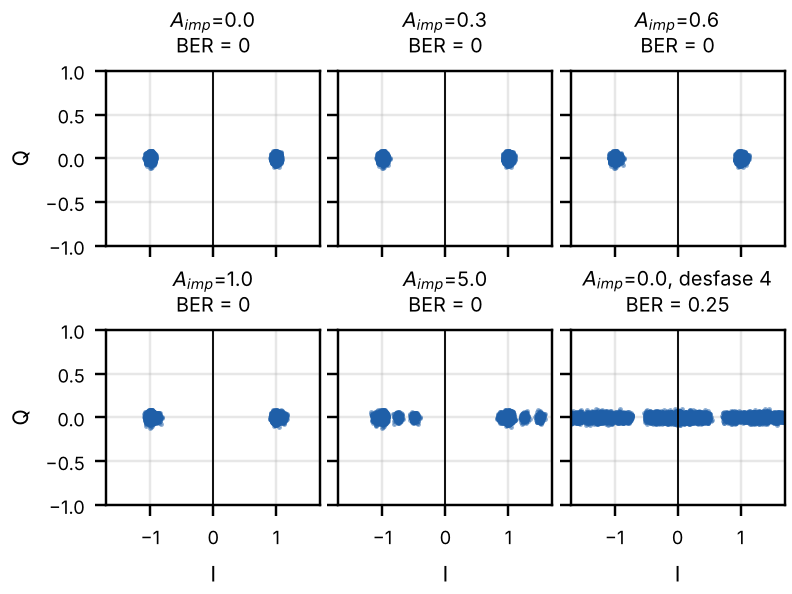
\includegraphics[width=\linewidth]{Figuras/constelaciones.png}
    \caption{Constelación recuperada (una muestra por símbolo): condición ideal, cada amplitud de impulso con AWGN 0.10 y, en el último panel, el efecto de muestrear con 4 muestras de desfase.}
    \label{fig:const}
\end{figure}

La Tabla~\ref{tab:fase2} resume la validación. En todas las pruebas los bits recuperados coinciden con los transmitidos una vez se compensan los 11 bits de retardo (Fig.~\ref{fig:bits}). El margen mínimo, es decir el menor $|I|$ observado en las muestras de decisión, cae de 0.88 a 0.40 cuando $A_{imp}$ pasa de 0 a 5. Sin AWGN, el primer error aparecería cuando $0.100\,A_{imp}>1$, es decir para $A_{imp}\approx10$.

\begin{table}[H]
    \centering
    \caption{Validación del receptor (AWGN 0.10 salvo en la prueba 0): BER medida en el flujograma (ventana de $10^5$ bits) y margen mínimo de la simulación ($2\times10^5$ bits)}
    \label{tab:fase2}
    \footnotesize
    \begin{tabular}{@{}lccc@{}}
        \toprule
        \textbf{Prueba} & $\mathbf{A_{imp}}$ & \textbf{BER} & \textbf{Margen mínimo $|I|$} \\
        \midrule
        0 (ideal, sin ruido) & 0.0 & 0 & 0.99 \\
        A (referencia) & 0.0 & 0 & 0.88 \\
        B (suave) & 0.3 & 0 & 0.88 \\
        C (media) & 0.6 & 0 & 0.85 \\
        D (fuerte) & 1.0 & 0 & 0.81 \\
        E (robustez) & 5.0 & 0 & 0.40 \\
        F (desfase 4) & 0.0 & 0.2498 & -- \\
        \bottomrule
    \end{tabular}
\end{table}

\begin{figure}[H]
    \centering
    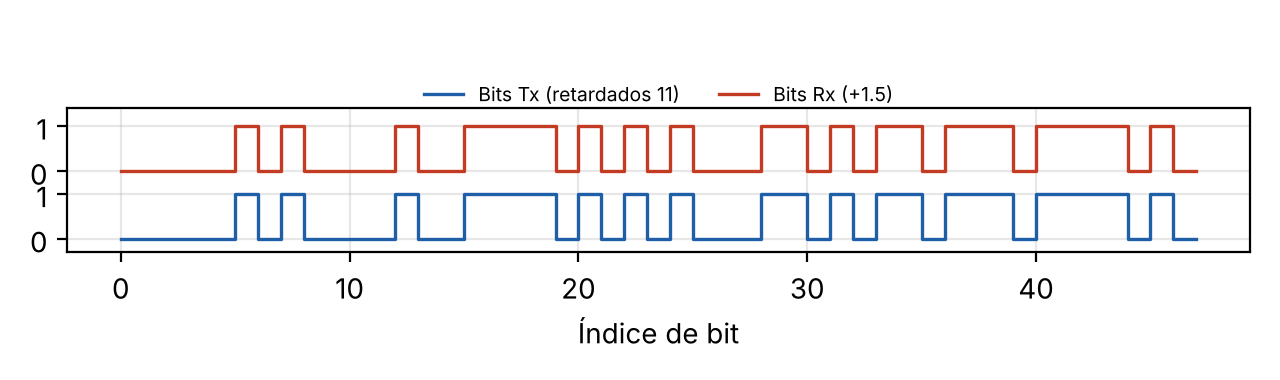
\includegraphics[width=\linewidth]{Figuras/bits_tx_rx.png}
    \caption{Bits transmitidos (abajo, retrasados 11 bits) y bits recuperados (arriba, desplazados $+1.5$) con $A_{imp}=1$.}
    \label{fig:bits}
\end{figure}

El instante de muestreo resultó tan determinante como el canal. Con el desfase correcto (0 muestras) el margen es 0.88; con 2 muestras de error baja a 0.18, y con 4 muestras ---el cruce del ojo--- la BER sube a 0.25 sin que el canal haya cambiado. Este resultado justifica calcular el retardo total del enlace (88 muestras, 11 símbolos) antes de fijar el muestreo y, en hardware, recuperar el reloj de forma adaptativa.

\subsection{Fase 3: configuración de la interfaz SDR}
En la tercera fase el enlace se llevó a flujogramas para HackRF One y USRP (Fig.~\ref{fig:fase3flujos}). El transmisor conserva la fuente PRBS-15, la codificación diferencial, el mapeo BPSK y el RRC de la Fase~2; después del RRC se agregan un factor de amplitud digital (para mantener el pico por debajo de 1 y no saturar el conversor), la adaptación de tasa a la del radio, el desplazamiento del oscilador y el bloque del radio. El receptor invierte el camino: corrige el desplazamiento del oscilador, vuelve a 256~kS/s y suma de forma digital el mismo tren de impulsos del proyecto, para reproducir el escenario sobre la señal real. Como los dos radios tienen osciladores independientes, agrega control automático de ganancia, lazo de frecuencia de borde de banda (corrige el offset entre osciladores), sincronización de reloj con banco polifásico de filtros RRC (que cumple además la función del filtro acoplado y elige el instante de muestreo de forma adaptativa) y lazo de Costas de orden 2, antes de la misma decisión y decodificación diferencial. Un filtro RRC adicional alimenta solo el diagrama de ojo de diagnóstico. Se eliminó el bloque de regulación de ritmo y el modelo de canal: con hardware, el radio fija el ritmo de muestras y el canal es el medio físico.

\begin{figure*}[!t]
    \centering
    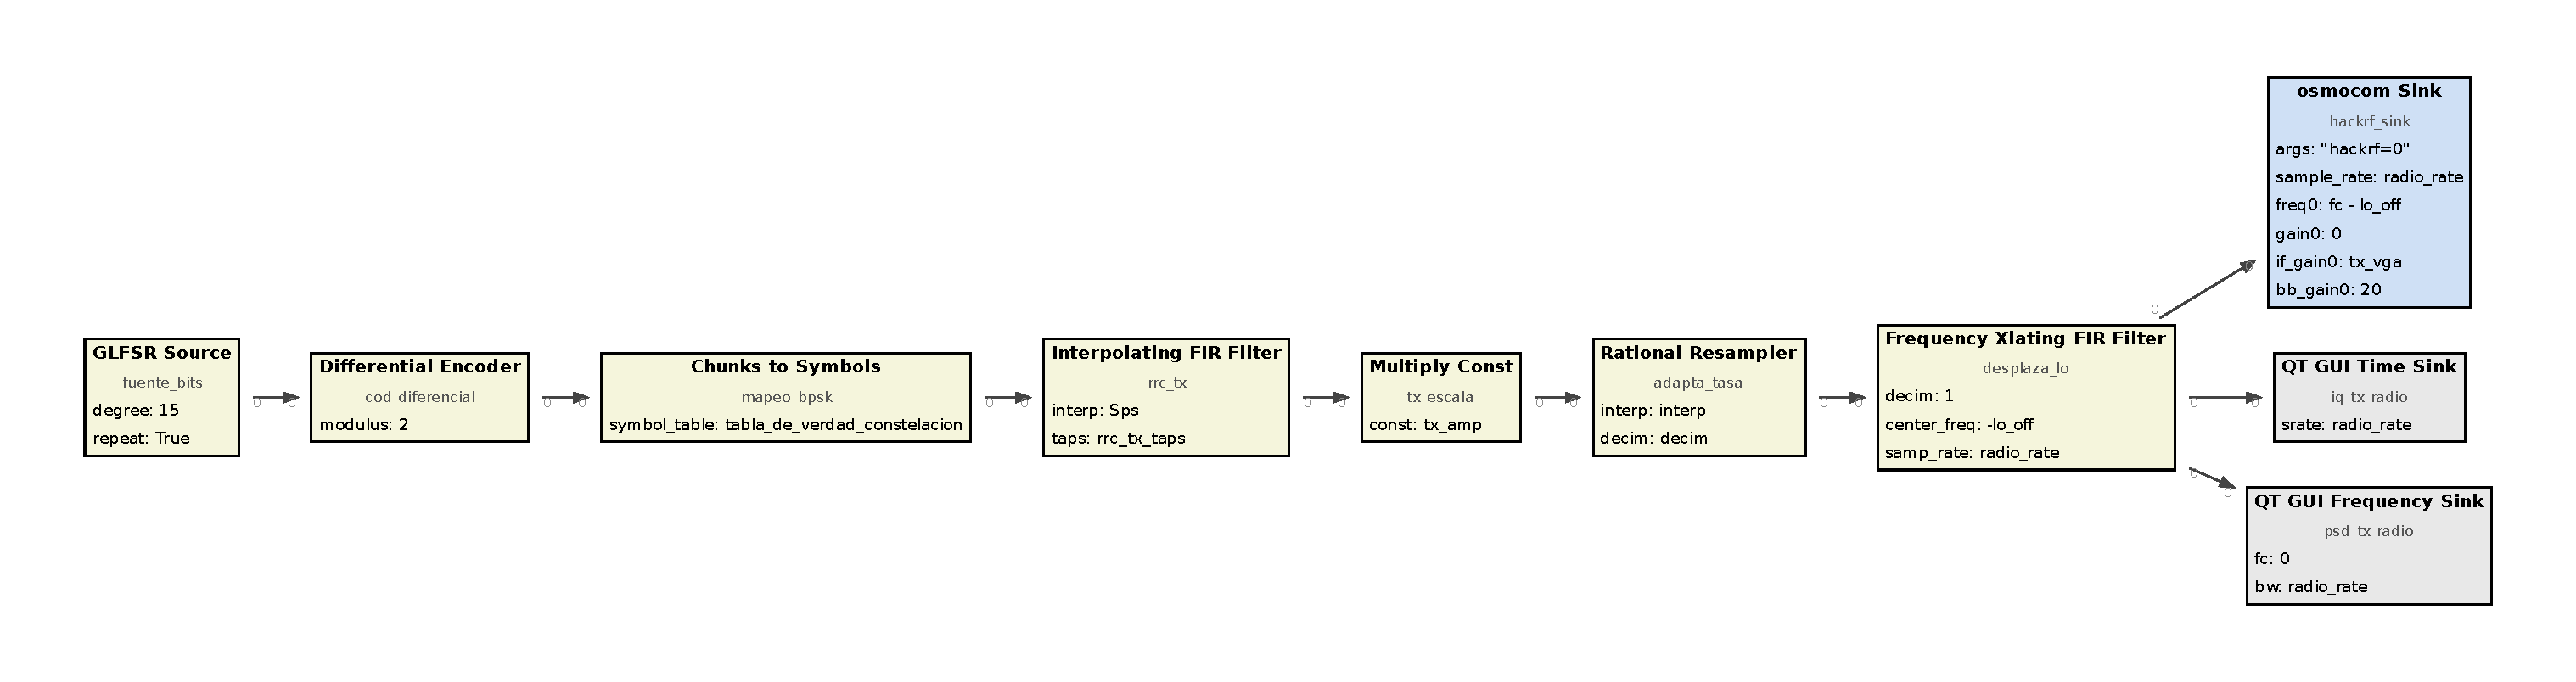
\includegraphics[width=0.92\textwidth]{Figuras/fase3_tx.pdf}\\[2mm]
    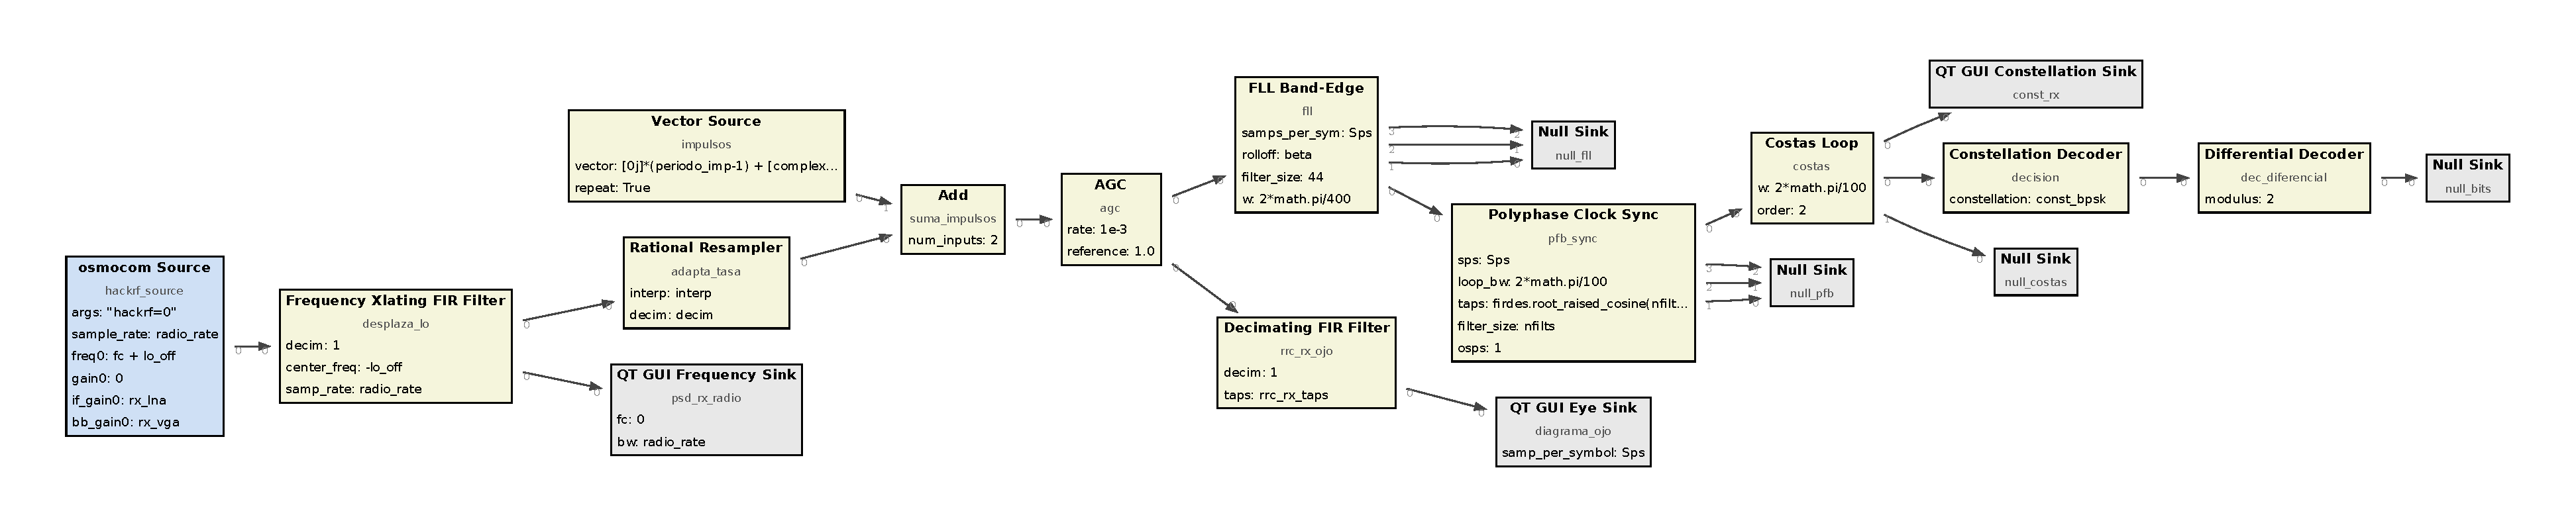
\includegraphics[width=\textwidth]{Figuras/fase3_rx.pdf}
    \caption{Flujogramas de la Fase~3 para HackRF One, con los parámetros principales de cada bloque tomados de los archivos \texttt{.grc}. Arriba, transmisor: PRBS, codificación diferencial, BPSK, RRC, amplitud, remuestreo a 2~MS/s, desplazamiento del oscilador y \textit{osmocom Sink}. Abajo, receptor: \textit{osmocom Source}, corrección del oscilador, regreso a 256~kS/s, suma de impulsos, AGC, FLL, sincronización de reloj polifásica, Costas, decisión y decodificación diferencial. Las versiones para USRP solo cambian el bloque del radio (UHD) y la tasa (1~MS/s).}
    \label{fig:fase3flujos}
\end{figure*}


La Fig.~\ref{fig:bloques} muestra la configuración de los bloques de radio y la Tabla~\ref{tab:sdr} (Anexo~\ref{app:sdr}) justifica cada parámetro. La separación entre diseño y hardware es la idea central de esta fase. Modulación, $R_s$, $R_b$, SPS, $\beta$, span, mapeo y decisión pertenecen al diseño de comunicaciones y no cambiaron. Frecuencia central (960~MHz), tasa del radio (2~MS/s en HackRF, 1~MS/s en USRP), remuestreo racional ($\times125/16$ y $\times125/32$), ganancias, ancho de banda RF, puerto, reloj y desplazamiento de 200~kHz del oscilador pertenecen a la interfaz. Así, cualquier diferencia entre la simulación y la medición en hardware se puede atribuir a la interfaz y al medio físico, y no a un cambio del diseño.

\begin{figure*}[t]
    \centering
    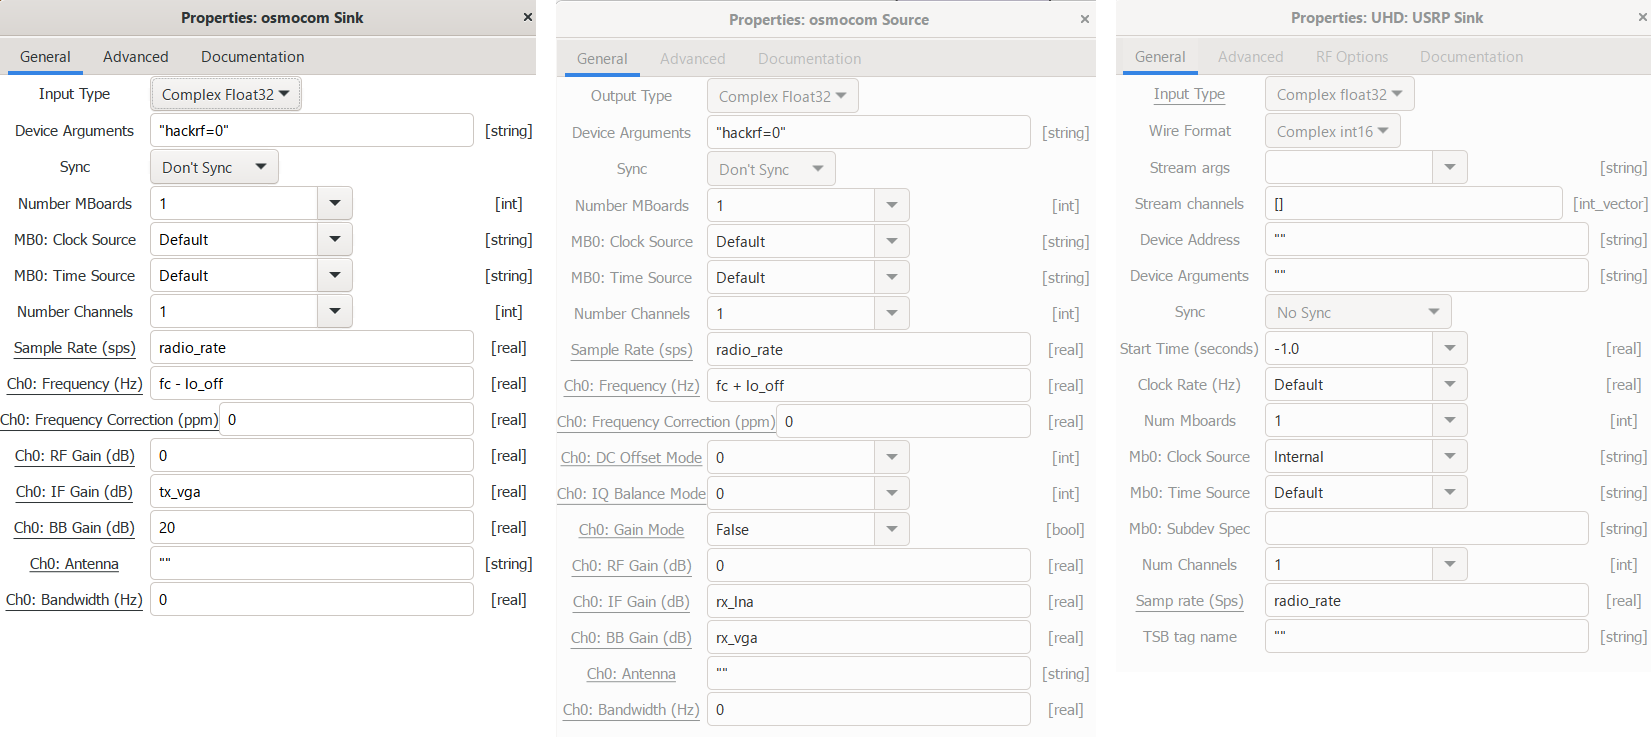
\includegraphics[width=\textwidth]{Figuras/bloques_radio.png}
    \caption{Configuración de los bloques de radio: Osmocom Sink (transmisor HackRF), Osmocom Source (receptor HackRF) y UHD: USRP Sink (transmisor USRP).}
    \label{fig:bloques}
\end{figure*}

En el Osmocom Sink la frecuencia es \texttt{fc - lo\_off}, la tasa \texttt{radio\_rate}, la ganancia de RF (amplificador) 0 y la ganancia IF \texttt{tx\_vga}; el campo BB no tiene efecto en transmisión con HackRF. En el Osmocom Source la frecuencia es \texttt{fc + lo\_off}, la ganancia IF corresponde al LNA (\texttt{rx\_lna}) y la BB al VGA (\texttt{rx\_vga}), con el control automático de ganancia del radio desactivado para que el nivel sea repetible. En ambos, el ancho de banda 0 deja que el driver elija el filtro analógico. En el USRP Sink la dirección vacía toma el primer equipo encontrado, el reloj es interno y la frecuencia, la ganancia y la antena (TX/RX) se fijan en la pestaña de opciones de RF.

\begin{figure*}[t]
    \centering
    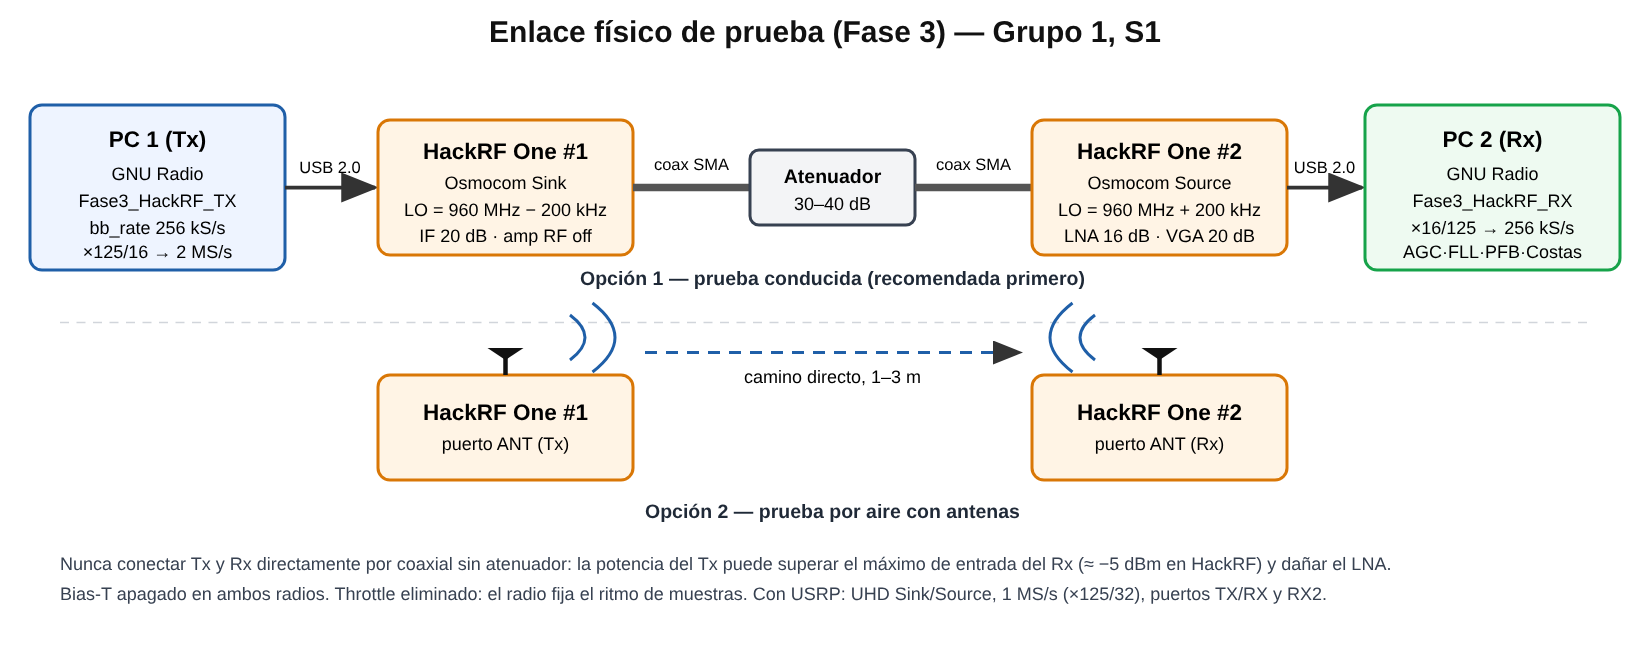
\includegraphics[width=0.9\textwidth]{Figuras/enlace_fisico.png}
    \caption{Montaje del enlace físico de prueba: por cable con atenuador (opción 1) o por aire con antenas (opción 2).}
    \label{fig:enlace}
\end{figure*}

La Fig.~\ref{fig:enlace} muestra el montaje previsto. La primera prueba se hace por cable con al menos 30~dB de atenuación, porque la potencia del transmisor puede superar el máximo de entrada del receptor (unos $-5$~dBm en HackRF). La tasa de bits no depende del radio: $256\,000\times125/16=2\times10^6$ muestras/s, y la señal de 43~kHz queda muy por debajo del ancho de banda del radio. Para medir la BER en hardware, \texttt{delay\_bits} se calibra primero con el bloque del Anexo~\ref{app:retardo}, porque el retardo deja de ser 11 bits: depende de los remuestreadores, de la sincronización y del instante en que arrancan el transmisor y el receptor. Los errores encontrados durante la configuración y su solución están en la Tabla~\ref{tab:errores}.

\subsection{Fase 4: validación con curvas BER}
Las curvas de la Fig.~\ref{fig:ber} se midieron en los flujogramas de la Fase~4 con el instrumento del curso, con los parámetros de la Tabla~\ref{tab:instr}: \texttt{e\_EbN0\_Sweep} se ubicó a la salida del canal, justo antes del filtro acoplado, y \texttt{e\_BER\_Curve} recibe los bits de la fuente PRBS (entrada 0) y los bits a la salida del decodificador diferencial (entrada 1) (Anexo~\ref{app:fase4}).

\begin{table}[H]
    \centering
    \caption{Parámetros del instrumento BER}
    \label{tab:instr}
    \footnotesize
    \begin{tabular}{@{}ll@{}}
        \toprule
        \textbf{Parámetro} & \textbf{Valor} \\
        \midrule
        $R_b$ & 32\,000 b/s \\
        \texttt{bb\_rate} (entrada del receptor) & 256\,000 muestras/s \\
        \texttt{EbN0\_min} / \texttt{EbN0\_max} / \texttt{EbN0\_step} & 0 / 14 / 1 dB \\
        \texttt{bits\_por\_punto} / \texttt{bits\_guardia} & 100\,000 / 1000 \\
        \texttt{delay\_bits} & 11 \\
        \texttt{update\_every} & 1000 \\
        \bottomrule
    \end{tabular}
\end{table}

Para alinear Tx y Rx se partió del retardo calculado en la Fase~2 (88 muestras = 11 símbolos) y se verificó con el bloque \texttt{e\_Busca\_Retardo}, que correlaciona ambas secuencias en una condición limpia. Cada flujograma corrió 4 minutos, unas 15 vueltas del barrido, lo que da entre $1.4$ y $1.6\times10^6$ bits por punto. Antes de medir, el bloque \texttt{e\_Busca\_Retardo} confirmó el retardo de 11 bits con correlación $+1.000$ y BER nula en los puntos de alta $E_b/N_0$.

Sin impulsos, la curva coincide con la de BPSK con codificación diferencial: $E_b/N_0=7.30$~dB para BER $=10^{-3}$, frente a 7.33~dB teóricos y 6.79~dB de BPSK coherente sin codificación diferencial. Esa diferencia de unos 0.5~dB es el costo de resolver la ambigüedad de fase, porque un error de símbolo produce dos errores de bit consecutivos. Con $A_{imp}=1$ la curva prácticamente no se distingue de la referencia (7.38~dB), lo que confirma lo observado en el ojo. Los pocos errores registrados a 14~dB en esas dos curvas (unos 10 en $1.4\times10^6$ bits) no son del enlace: aparecen en el salto de 14 a 0~dB al reiniciar el barrido, cuando algunos bits del final del punto de 14~dB ya reciben el ruido del punto de 0~dB. A 12 y 13~dB no hubo errores.

\begin{figure}[H]
    \centering
    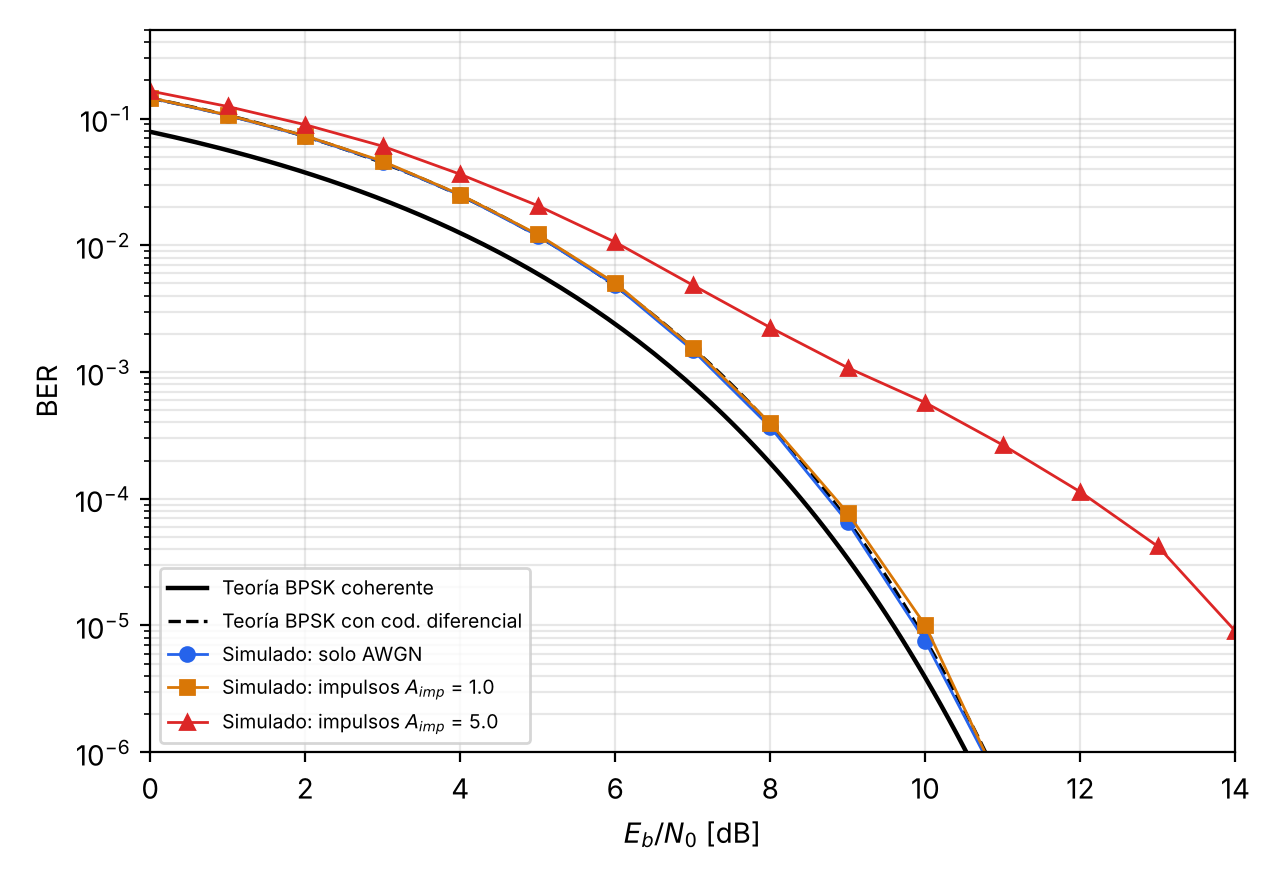
\includegraphics[width=\linewidth]{Figuras/curva_ber.png}
    \caption{BER frente a $E_b/N_0$ medida en los flujogramas de la Fase~4 ($A_{imp}=0$, 1 y 5) junto con la teoría de BPSK coherente y con codificación diferencial. Los puntos vacíos a 14~dB son errores causados por el reinicio del barrido.}
    \label{fig:ber}
\end{figure}

Con $A_{imp}=5$ la curva se separa: requiere 9.17~dB para BER $=10^{-3}$ (1.8~dB más que la referencia) y, en lugar de caer en forma de cascada, decrece lentamente: $2.7\times10^{-4}$ a 11~dB y $1.7\times10^{-5}$ a 14~dB. El comportamiento se explica con un modelo simple. De cada 32 símbolos, el más cercano al impulso pierde la mitad de su distancia al umbral ($1-0.100\times5=0.5$), es decir, unos 6~dB de relación señal a ruido, y a alta $E_b/N_0$ son esos símbolos los que producen casi todos los errores. Promediando la probabilidad de error de cada símbolo según su desplazamiento se obtienen $1.1\times10^{-3}$ a 9~dB y $2.7\times10^{-4}$ a 11~dB; el flujograma midió $1.12\times10^{-3}$ y $2.71\times10^{-4}$, y la simulación numérica del mismo enlace dio valores iguales. Parte de la penalización, unos 0.4~dB, es aparente: el instrumento mide la potencia recibida incluyendo los impulsos y asigna ruido con base en ella.

\begin{table}[H]
    \centering
    \caption{$E_b/N_0$ requerido para BER $=10^{-3}$}
    \label{tab:ber}
    \footnotesize
    \begin{tabular}{@{}lcc@{}}
        \toprule
        \textbf{Condición} & $\mathbf{E_b/N_0}$ \textbf{[dB]} & \textbf{Penalización [dB]} \\
        \midrule
        Teoría BPSK coherente & 6.79 & -- \\
        Teoría con cod. diferencial & 7.33 & referencia \\
        Medido, sin impulsos & 7.30 & $-0.03$ \\
        Medido, $A_{imp}=1$ & 7.38 & $+0.05$ \\
        Medido, $A_{imp}=5$ & 9.17 & $+1.84$ \\
        \bottomrule
    \end{tabular}
\end{table}


La curva medida sin impulsos es la referencia contra la que se compara la curva experimental con el radio, con el criterio del curso de una penalización máxima de 2~dB en BER $=10^{-3}$.

% RESULTADOS Y DISCUSIÓN (Datos, figuras y tablas)
% Presentación de figuras, tablas y datos importantes (como PSD, diagramas de ojo, constelaciones y curvas BER vs SNR) completamente citados y explicados dentro del texto.

\section{Conclusiones}
\label{sec:conclusiones}

\begin{itemize}
    \item El requerimiento de telemetría (16~kb/s útiles con margen 2:1) se cubrió con BPSK a $R_s=32$~ksym/s, SPS~$=8$ y conformación RRC con $\beta=0.35$. El ancho de banda ocupado bajó de unos 64~kHz con pulso rectangular a 43.2~kHz, sin interferencia intersimbólica en los instantes de decisión.
    \item El ruido impulsivo periódico se identifica en el dominio del tiempo y en la constelación, pero casi no en la PSD. Su potencia media es pequeña ($A_{imp}^2/256$) y solo se manifiesta como un aumento del piso y un peine de líneas a la frecuencia de repetición de 1~kHz. Para este tipo de perturbación, la PSD no es un buen indicador del riesgo de error.
    \item El filtro acoplado fue la principal defensa contra los impulsos: en los instantes de decisión reduce un impulso de una muestra a $0.100\,A_{imp}$. Con AWGN de amplitud 0.10, la BER fue cero en todas las pruebas ($A_{imp}$ hasta 5), aunque el margen de decisión bajó de 0.88 a 0.40. En la fase de canal, en cambio, con pulso rectangular y sin filtro acoplado, $A_{imp}=1$ bastaba para llevar símbolos al umbral.
    \item El instante de muestreo resultó crítico: un error de medio símbolo eleva la BER a 0.25 aunque el canal no cambie. Calcular el retardo total del enlace (88 muestras) y, en hardware, recuperar el reloj y calibrar el retardo de bits son condiciones necesarias para que la medición de BER tenga sentido.
    \item Sin impulsos, el enlace alcanza BER $=10^{-3}$ con $E_b/N_0=7.3$~dB, de acuerdo con la teoría de BPSK con codificación diferencial; esta cuesta unos 0.5~dB frente a BPSK coherente, a cambio de eliminar la ambigüedad de fase de 180° del receptor de hardware. Con $A_{imp}=1$ no hay penalización medible. Con $A_{imp}=5$ la penalización es de 1.8~dB y la curva decae lentamente, porque uno de cada 32 símbolos pierde la mitad de su distancia al umbral. Si la amplitud de los impulsos de la planta fuera de ese orden, convendría agregar codificación de canal con entrelazado o limitar la amplitud de las muestras antes del filtro acoplado.
    \item La migración a hardware se hizo sin cambiar ningún parámetro de diseño: modulación, $R_s$, SPS, $\beta$, span, mapeo y decisión se conservaron, y solo se agregaron la interfaz del radio (frecuencia central, tasa del radio, remuestreo, ganancias y desplazamiento del oscilador) y la sincronización de frecuencia, reloj y fase que exigen dos osciladores independientes. La codificación diferencial, cuyo costo medido fue de unos 0.5~dB, es la que permite resolver la ambigüedad de fase del lazo de portadora.
    \item Como trabajo futuro queda medir la curva BER del enlace BPSK propio con los radios, conectados por cable con atenuación, y compararla con la referencia simulada usando el criterio de penalización máxima de 2~dB en BER $=10^{-3}$. También queda evaluar codificación de canal con entrelazado y limitación de amplitud antes del filtro acoplado frente a impulsos de mayor amplitud.
\end{itemize}

% CONCLUSIONES (Sin mencionar herramientas como GitHub o GNU Radio)


% ANEXOS

\section{ANEXOS}

\subsection{Bloque de calibración del retardo Tx--Rx}
\label{app:retardo}

El bloque \texttt{e\_Busca\_Retardo} acumula bits transmitidos y recuperados, calcula su correlación cruzada mediante FFT y reporta el retardo que maximiza la coincidencia; una correlación negativa indica bits invertidos.

\begin{lstlisting}[style=bonito,
                   caption={Bloque \texttt{e\_Busca\_Retardo} para calibrar \texttt{delay\_bits}},
                   label={lst:retardo}]
import numpy as np
from gnuradio import gr

class blk(gr.sync_block):
    def __init__(self, n_bits=40000, max_lag=33000):
        gr.sync_block.__init__(self, name='e_Busca_Retardo',
                               in_sig=[np.int8, np.int8], out_sig=None)
        self.n_bits, self.max_lag = int(n_bits), int(max_lag)
        self.tx, self.rx = [], []
        self.total = self.n_bits + self.max_lag

    def work(self, input_items, output_items):
        self.tx.extend((input_items[0] & 1).tolist())
        self.rx.extend((input_items[1] & 1).tolist())
        if min(len(self.tx), len(self.rx)) >= self.total:
            tx = 2.0*np.array(self.tx[:self.total]) - 1.0
            rx = 2.0*np.array(self.rx[self.max_lag:self.total]) - 1.0
            n = 1 << int(np.ceil(np.log2(len(tx) + len(rx))))
            corr = np.fft.irfft(np.fft.rfft(tx, n) *
                                np.conj(np.fft.rfft(rx, n)), n)
            c = corr[:self.max_lag + 1][::-1] / len(rx)
            lag = int(np.argmax(np.abs(c)))
            print(f"delay_bits = {lag}  corr = {c[lag]:+.3f}")
            self.tx = self.tx[self.total:]
            self.rx = self.rx[self.total:]
        return len(input_items[0])
\end{lstlisting}

\subsection{Parámetros de la interfaz SDR}
\label{app:sdr}

\begin{table}[H]
    \centering
    \caption{Configuración de HackRF One y USRP}
    \label{tab:sdr}
    \footnotesize
    \setlength{\tabcolsep}{3pt}
    \begin{tabular}{@{}lcc@{}}
        \toprule
        \textbf{Parámetro} & \textbf{HackRF One} & \textbf{USRP} \\
        \midrule
        Bloque Tx / Rx & Osmocom Sink / Source & UHD Sink / Source \\
        Selección & \texttt{hackrf=0} & dirección o serial \\
        Tasa del radio & 2 MS/s & 1 MS/s \\
        Remuestreo Tx & $\times125/16$ & $\times125/32$ \\
        $f_c$ Tx / Rx & $f_c-200$ kHz / $f_c+200$ kHz & igual \\
        Ganancia Tx & IF 20 dB, amp. RF apagado & 20 dB \\
        Ganancia Rx & LNA 16 dB, VGA 20 dB & 30 dB \\
        Ancho de banda RF & automático & automático \\
        Antena & -- & TX/RX y RX2 \\
        Bias-T / reloj & apagado / interno & -- / interno \\
        \bottomrule
    \end{tabular}
\end{table}


\subsection{Arquitectura inicial: flujograma de la fase de canal}
\label{app:fase1}
\begin{figure}[H]
    \centering
    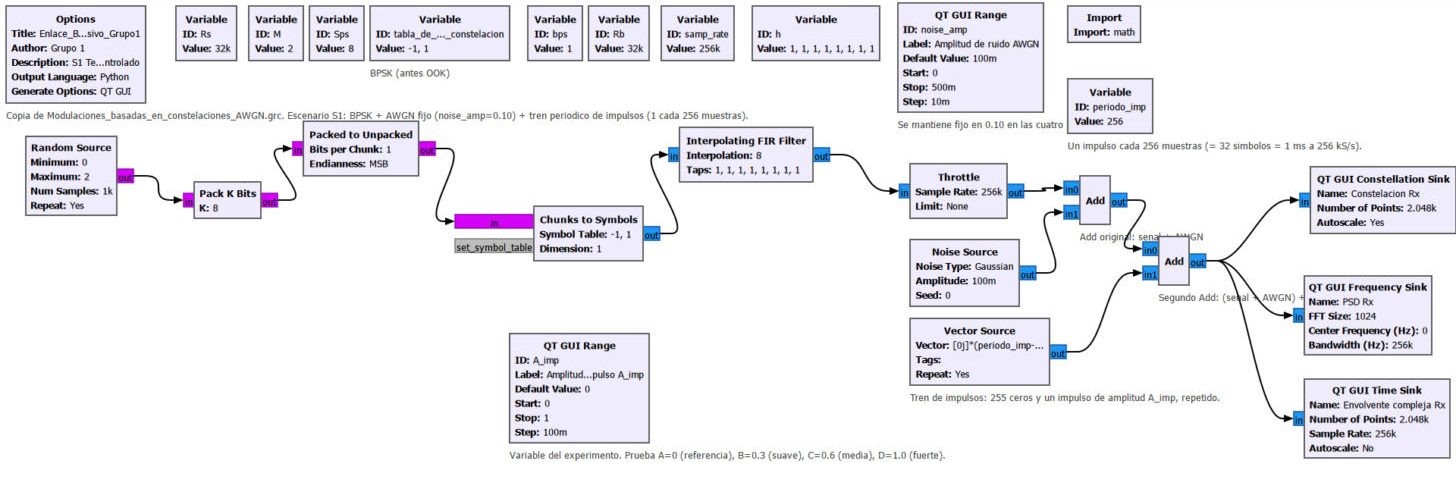
\includegraphics[width=\linewidth]{Figuras/grc_fase1.png}
    \caption{Flujograma de la fase de canal, construido a partir del archivo base del curso: BPSK con pulso rectangular, AWGN de amplitud 0.10 y tren de impulsos de amplitud $A_{imp}$ cada 256 muestras.}
    \label{fig:grc_fase1}
\end{figure}

\subsection{Capturas de GNU Radio por prueba (Fase 2)}
\label{app:capturas}
Las Figs.~\ref{fig:pA}--\ref{fig:pF} reúnen las capturas completas del flujograma de la Fase~2 para cada prueba, siempre con AWGN de amplitud 0.10. En cada figura, a la izquierda está la pestaña \emph{Transmisor y canal} (PSD de la salida del RRC y del canal, envolvente compleja del canal en 8~ms y plano I--Q sobremuestreado) y a la derecha la pestaña \emph{Receptor} (ojo de las componentes I y Q, constelación recuperada y salida del filtro acoplado en 2~ms). La Fig.~\ref{fig:validacion} reúne la pestaña \emph{Validación} de todas las pruebas.

\begin{figure*}[!t]
    \centering
    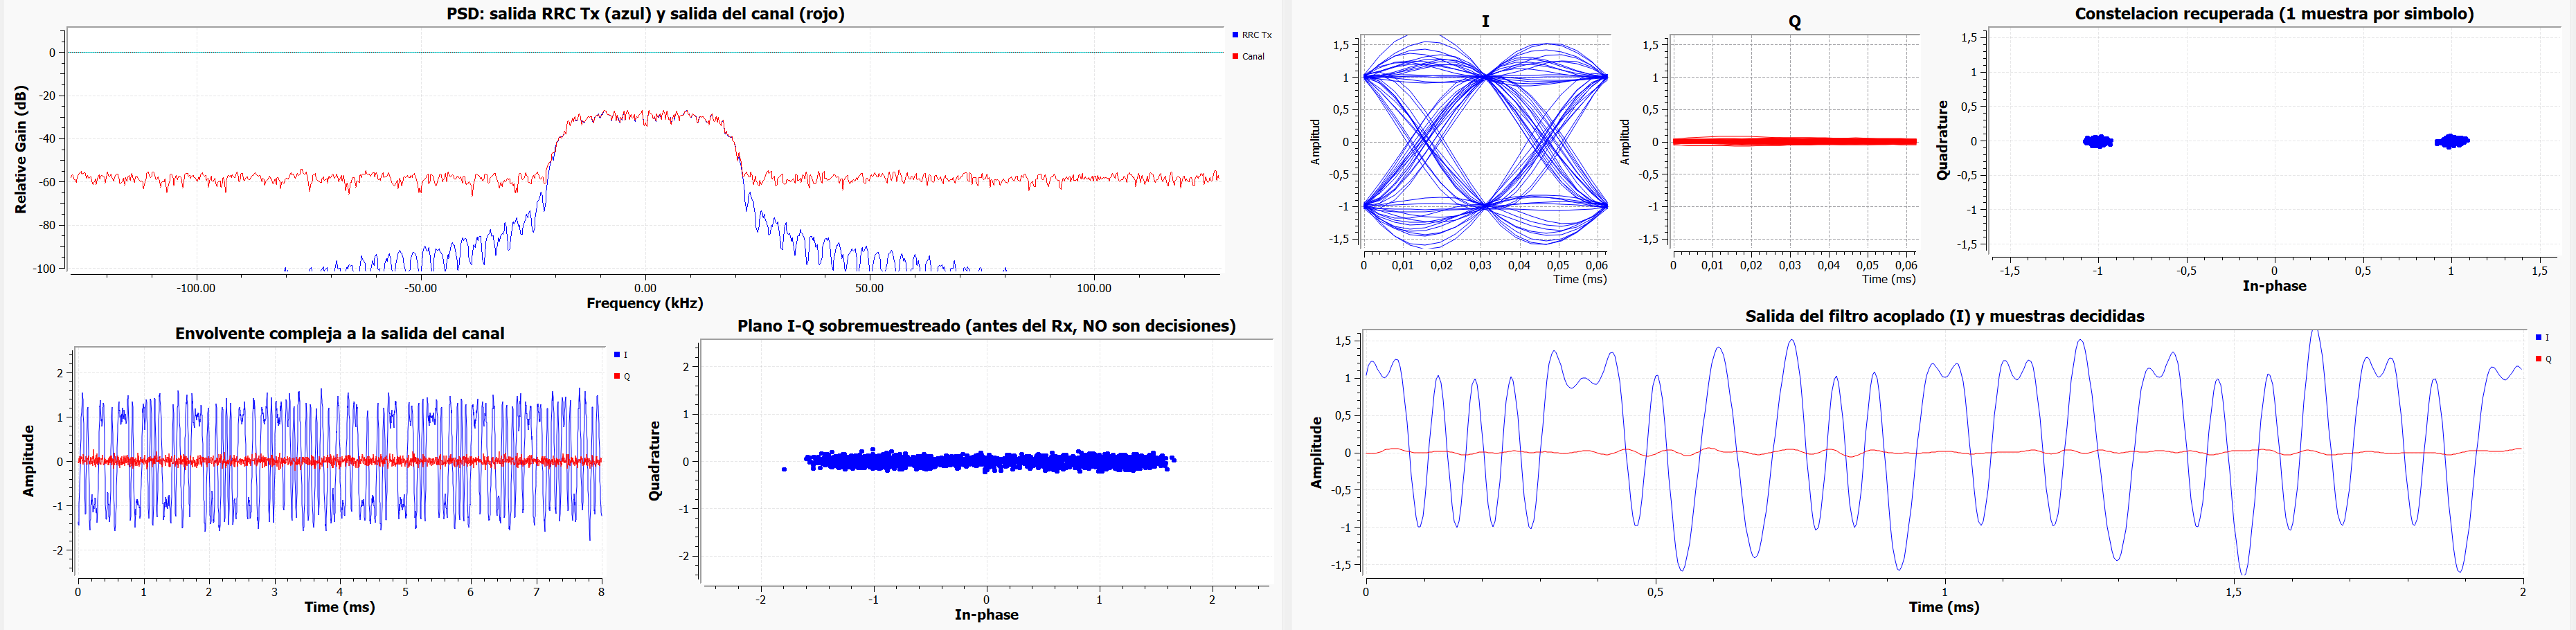
\includegraphics[width=\textwidth]{Figuras/prueba_A.png}
    \caption{Prueba A (referencia, $A_{imp}=0$).}
    \label{fig:pA}
\end{figure*}

\textbf{Prueba A.} Es la línea de base. La PSD del canal reproduce la de la señal RRC dentro de $\pm21.6$~kHz y fuera de ella queda el piso plano del AWGN. La envolvente solo tiene componente I, con niveles alrededor de $\pm1$, y el plano I--Q sobremuestreado es una franja horizontal: son las transiciones entre símbolos, no decisiones. En el receptor, el ojo está abierto por completo y las trayectorias convergen en $\pm1$ en los instantes de muestreo; la constelación recuperada son dos nubes compactas y la componente Q permanece en cero.

\begin{figure*}[!t]
    \centering
    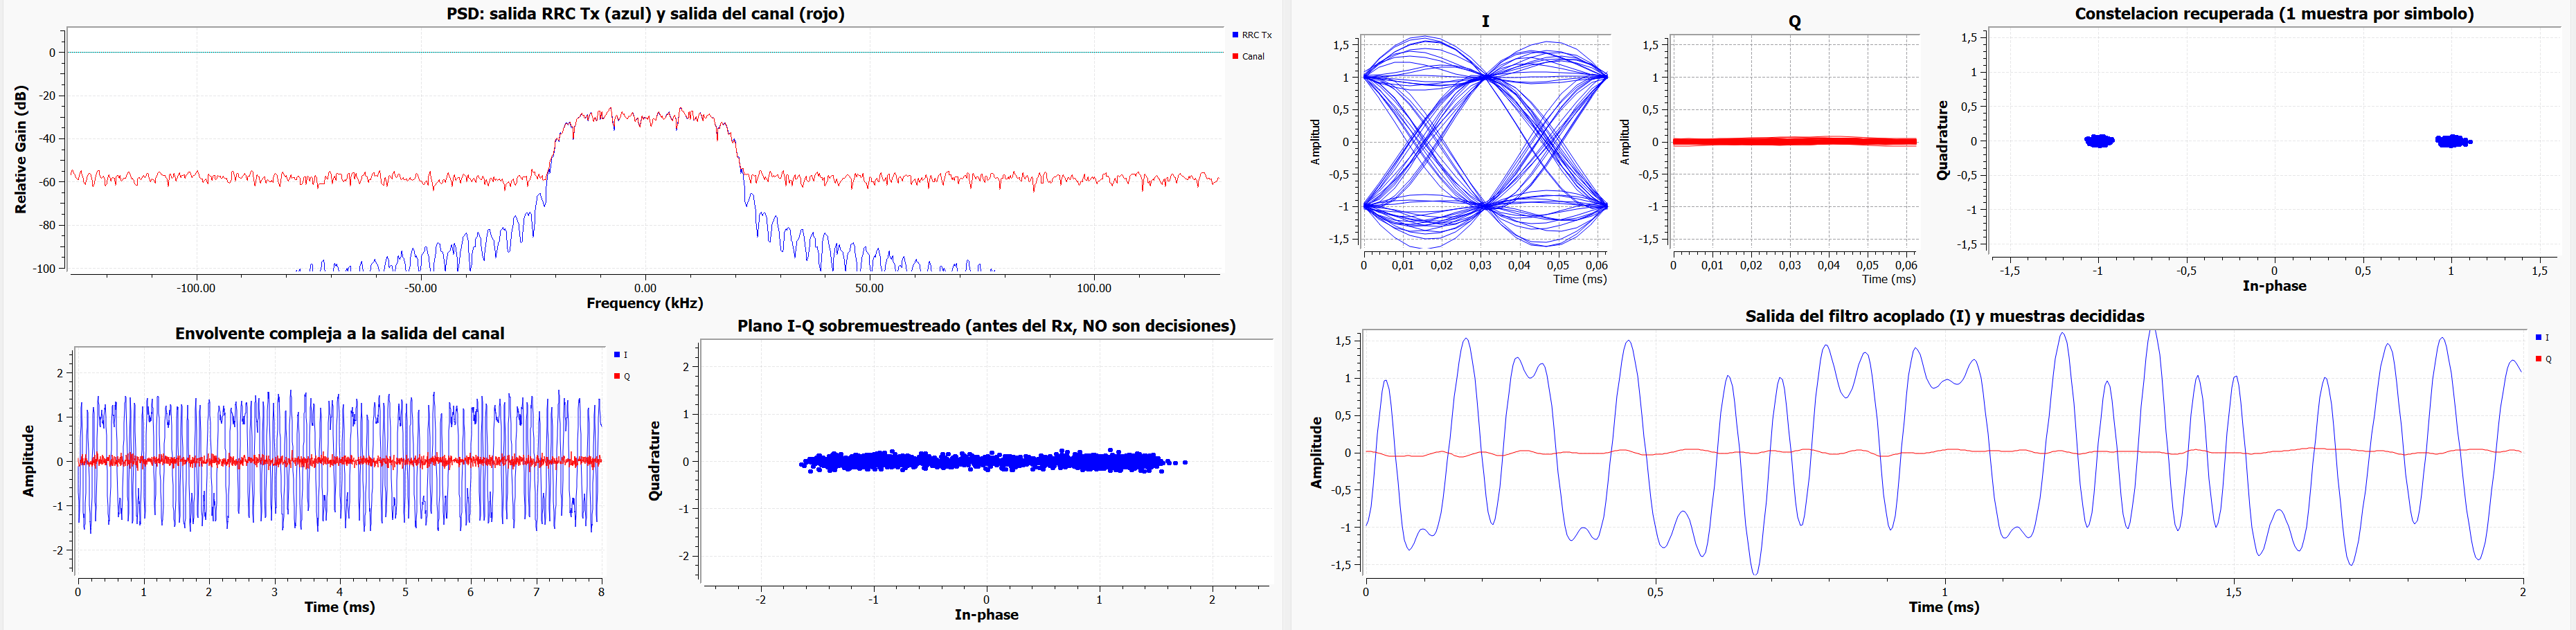
\includegraphics[width=\textwidth]{Figuras/prueba_B.png}
    \caption{Prueba B (perturbación suave, $A_{imp}=0.3$).}
    \label{fig:pB}
\end{figure*}

\textbf{Prueba B.} El tren de impulsos todavía no se distingue en la PSD ni en el ojo. En la envolvente aparecen picos de $\approx1.3$ cada milisegundo cuando el impulso coincide con un nivel positivo. Después del filtro acoplado el impulso se reduce a $0.03$ en la variable de decisión, por eso la constelación es igual a la de la referencia.

\begin{figure*}[!t]
    \centering
    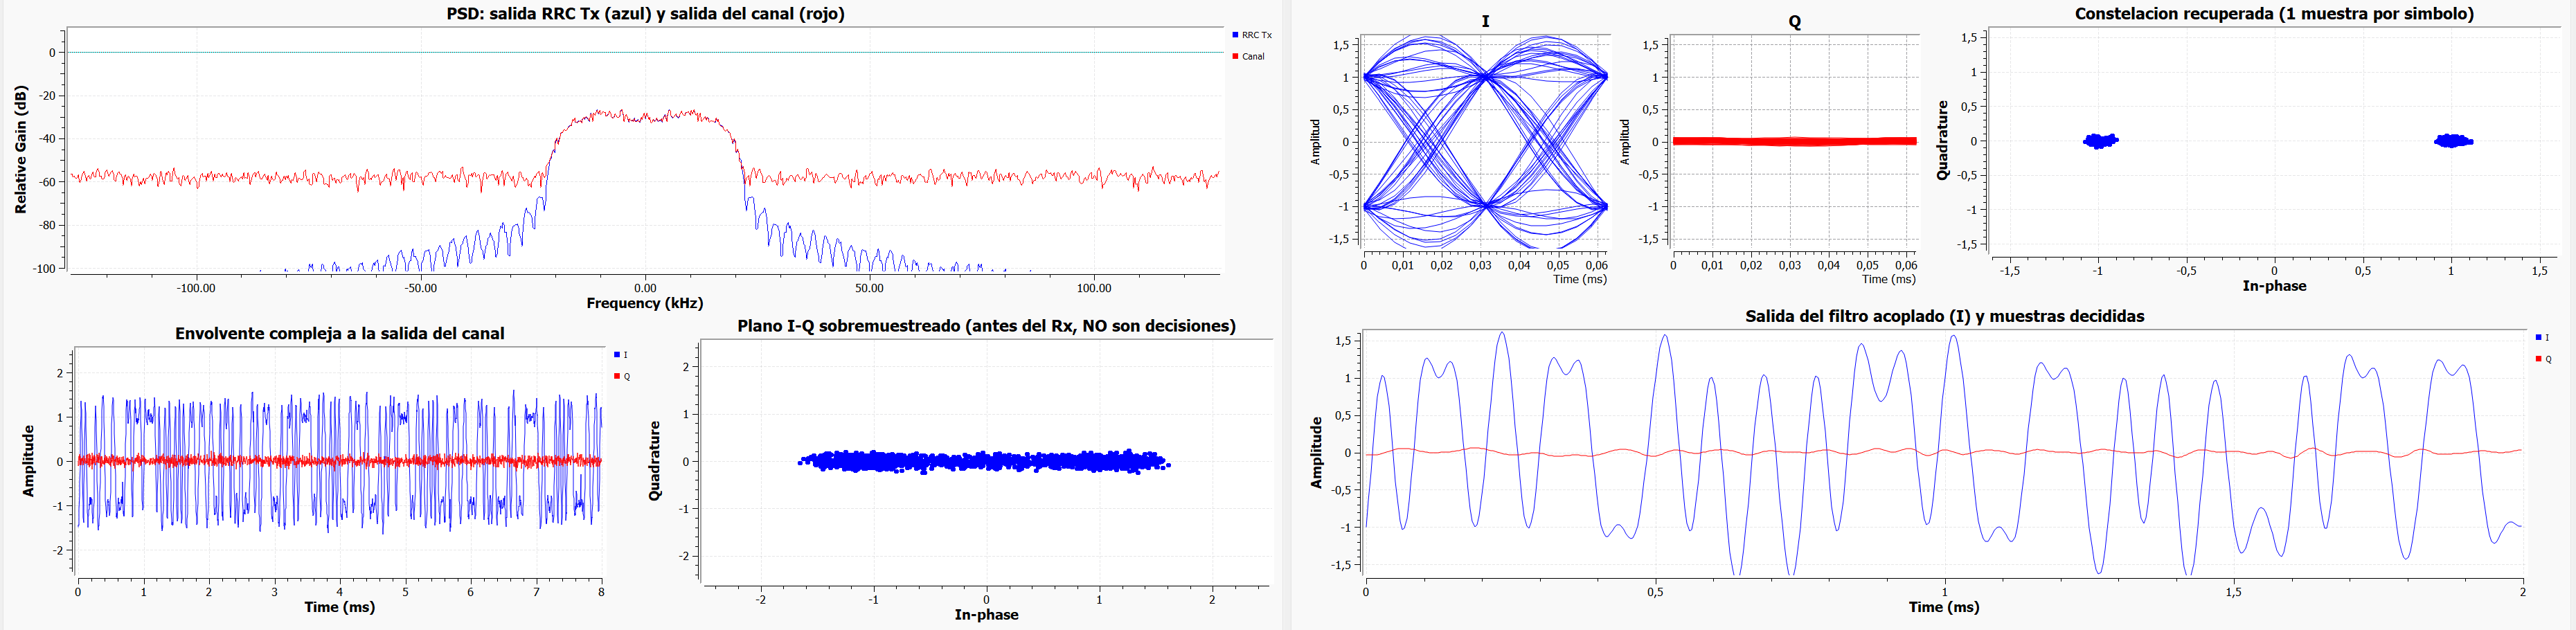
\includegraphics[width=\textwidth]{Figuras/prueba_C.png}
    \caption{Prueba C (perturbación media, $A_{imp}=0.6$).}
    \label{fig:pC}
\end{figure*}

\textbf{Prueba C.} Es la condición principal de análisis. Los picos de la envolvente llegan a $\approx1.6$ y el plano I--Q sobremuestreado se estira ligeramente hacia la derecha. El receptor sigue sin verse afectado: el desplazamiento máximo en la decisión es $0.06$, mucho menor que la distancia de 1 al umbral, y las nubes de la constelación siguen separadas.

\begin{figure*}[!t]
    \centering
    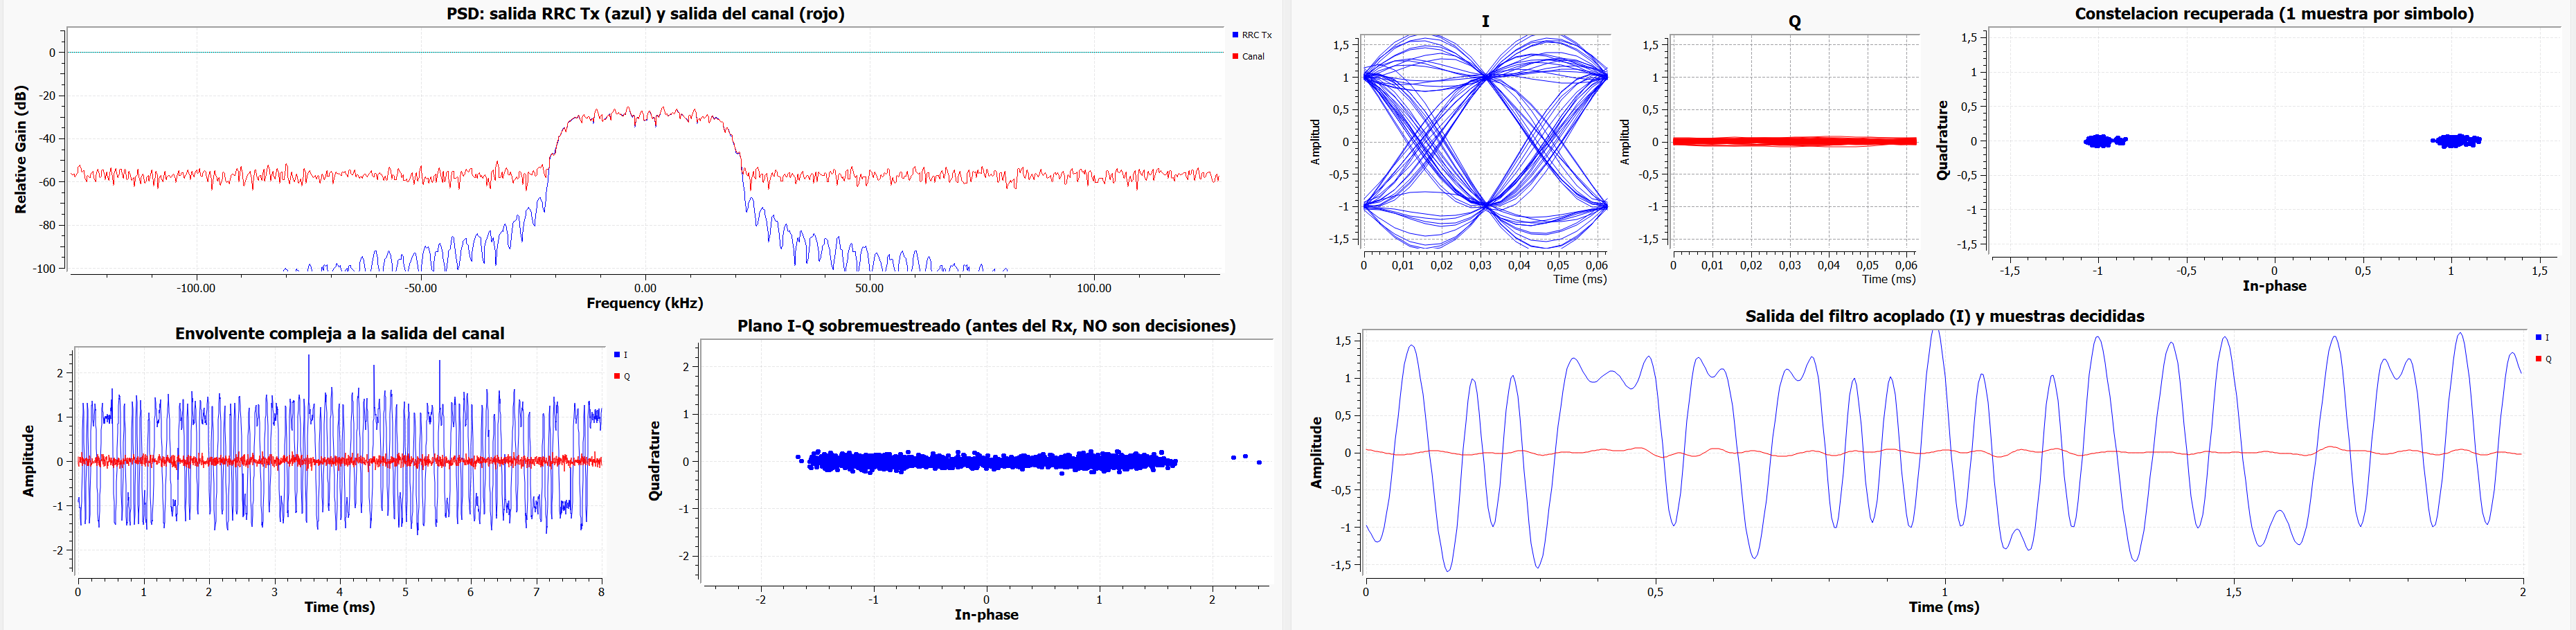
\includegraphics[width=\textwidth]{Figuras/prueba_D.png}
    \caption{Prueba D (perturbación fuerte, $A_{imp}=1.0$).}
    \label{fig:pD}
\end{figure*}

\textbf{Prueba D.} Los impulsos se ven con claridad en el tiempo, con picos que superan 2, y en el plano I--Q aparecen puntos aislados cerca de $I\approx2.3$, fuera de la franja de la señal. En la fase de canal, con pulso rectangular, esta amplitud llevaba los símbolos negativos al umbral. Con el filtro acoplado, la constelación solo muestra unas pocas muestras corridas $\approx0.1$ hacia la derecha y la BER sigue en cero.

\begin{figure*}[!t]
    \centering
    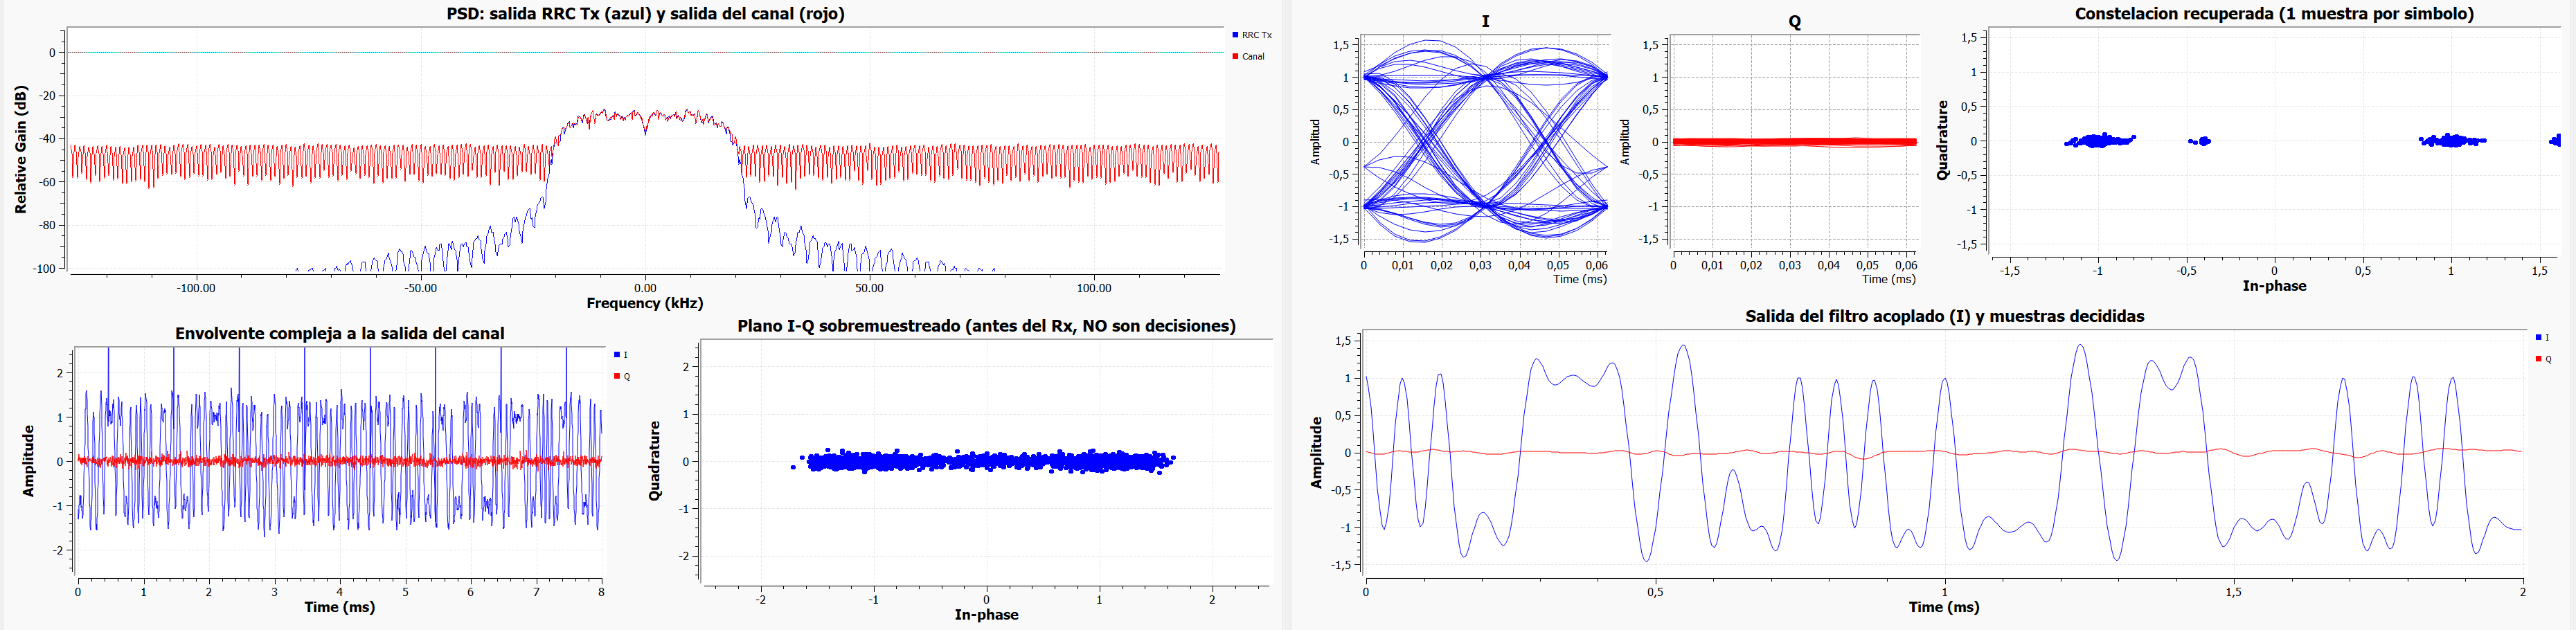
\includegraphics[width=\textwidth]{Figuras/prueba_E.png}
    \caption{Prueba E (robustez, $A_{imp}=5.0$).}
    \label{fig:pE}
\end{figure*}

\textbf{Prueba E.} Con impulsos cinco veces mayores que el símbolo, la PSD sí cambia: el piso sube unos 10~dB y aparece el peine de líneas cada 1~kHz. En la envolvente los picos salen de la escala. En el ojo aparecen trayectorias que se apartan del haz, y en la constelación surgen dos grupos aislados en $-0.5$ y $+1.5$, que son los símbolos que coinciden con un impulso. Aun así ninguna muestra cruza el umbral, porque el margen mínimo es 0.40, y la BER medida sigue en cero.

\begin{figure*}[!t]
    \centering
    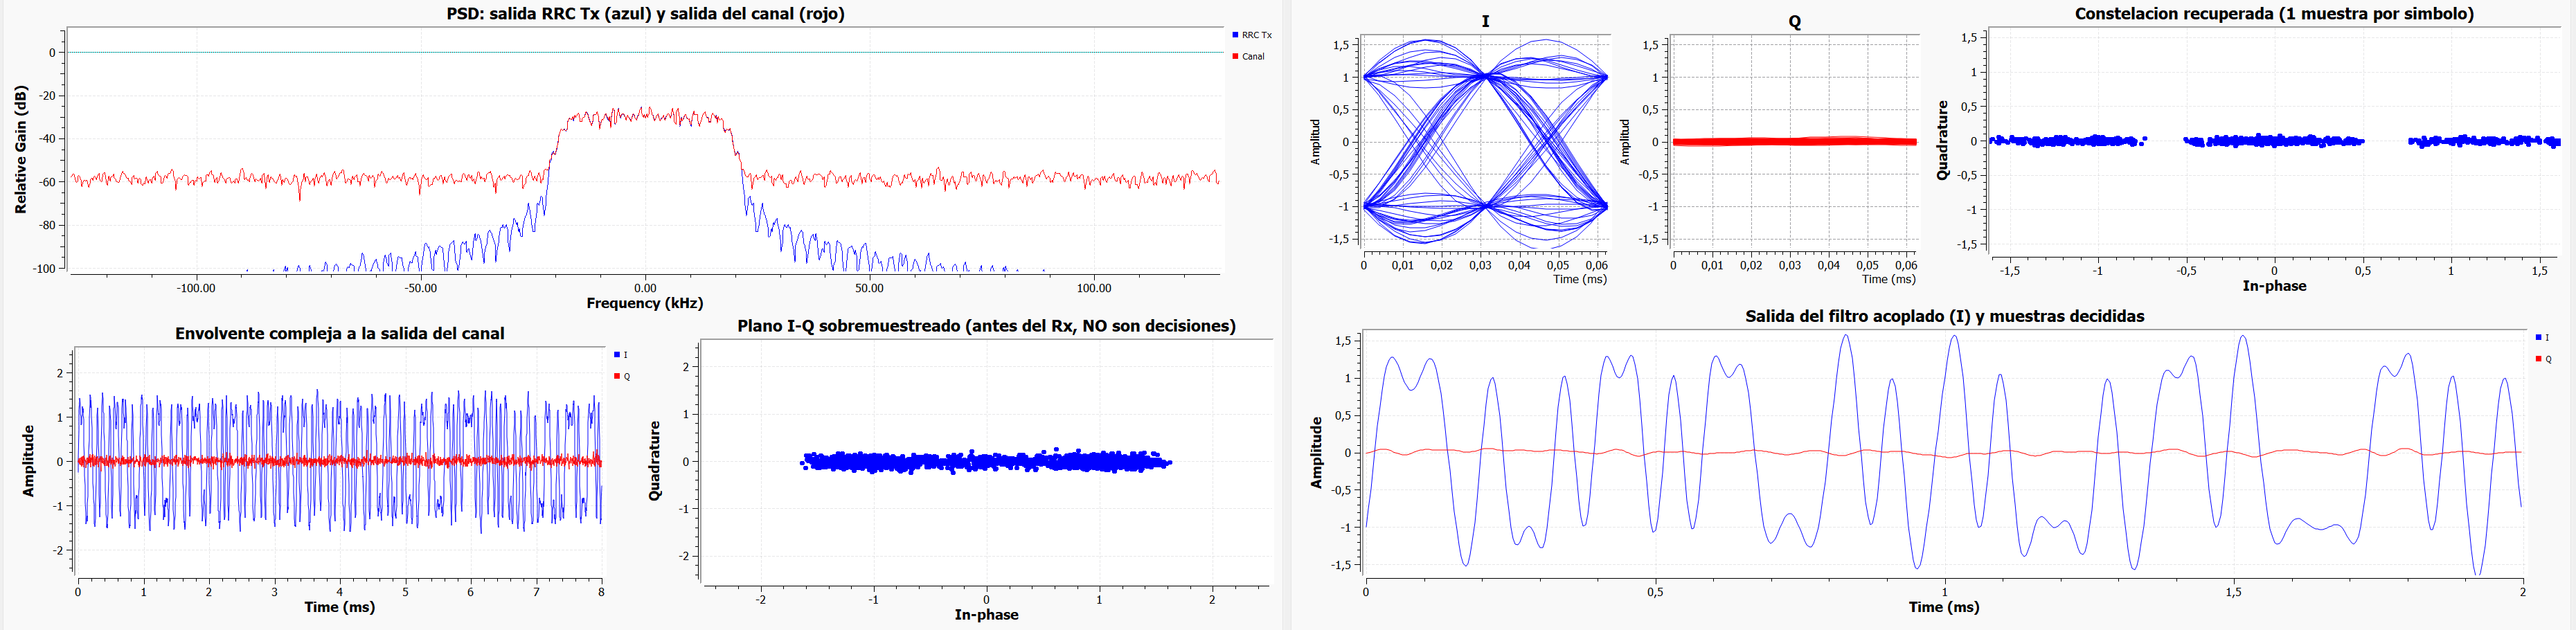
\includegraphics[width=\textwidth]{Figuras/prueba_F.png}
    \caption{Prueba F (referencia muestreada con 4 muestras de desfase).}
    \label{fig:pF}
\end{figure*}

\textbf{Prueba F.} El canal es el mismo de la referencia, como confirma la pestaña izquierda, idéntica a la de la Fig.~\ref{fig:pA}. Lo único que cambia es el instante de muestreo. La salida del filtro acoplado es igual, pero al tomar la muestra en el cruce del ojo la constelación se reparte a lo largo de todo el eje I, con valores cercanos a cero, y la BER sube a 0.2503. Esta prueba muestra que el receptor depende tanto de la sincronización como del canal.

\begin{figure*}[!t]
    \centering
    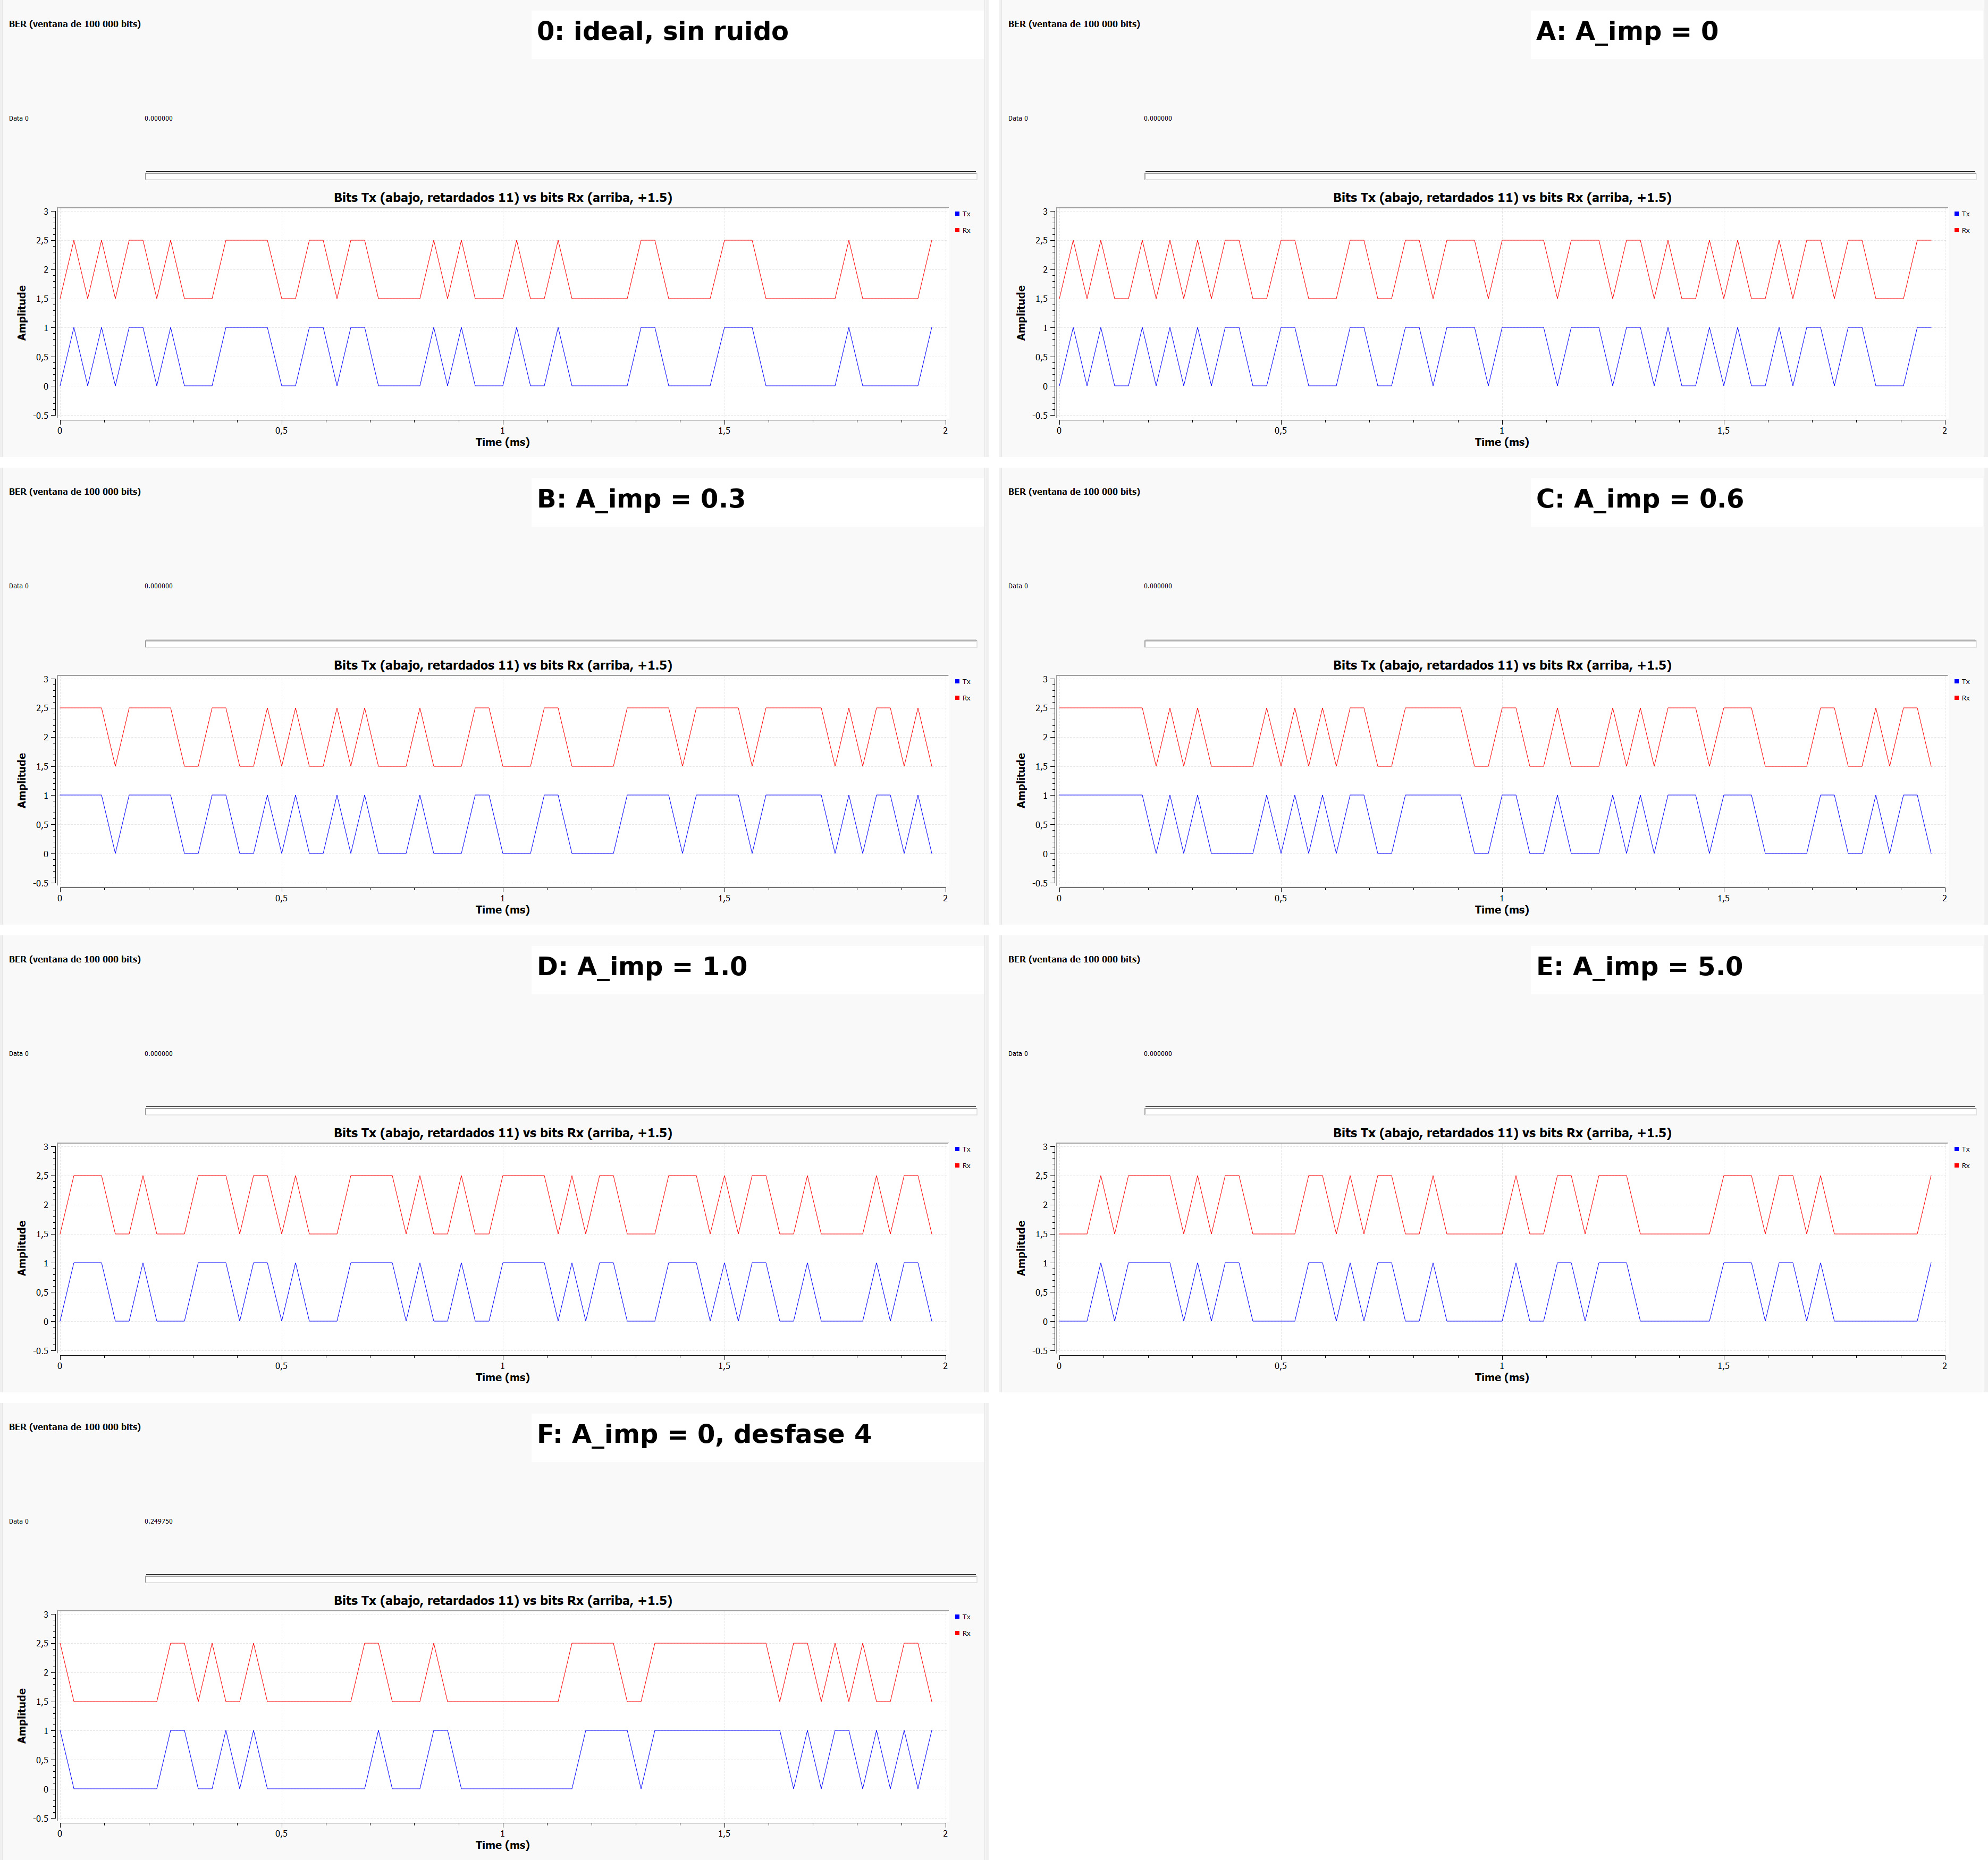
\includegraphics[width=0.92\textwidth]{Figuras/validacion_todas.png}
    \caption{Pestaña \emph{Validación} de las seis pruebas: BER en una ventana de $10^5$ bits y bits transmitidos (abajo, retrasados 11 bits) frente a bits recuperados (arriba, desplazados $+1.5$).}
    \label{fig:validacion}
\end{figure*}
\textbf{Validación.} En las pruebas A a E la BER de la ventana es 0.000000 y las dos secuencias de bits son idénticas, desplazadas solo por el retardo de 11 bits ya compensado. En la prueba F la BER es 0.2503 y se ven bits recuperados que no coinciden con los transmitidos.

\subsection{Ventanas de las curvas BER (Fase 4)}
\label{app:ventanas}
\begin{figure*}[!t]
    \centering
    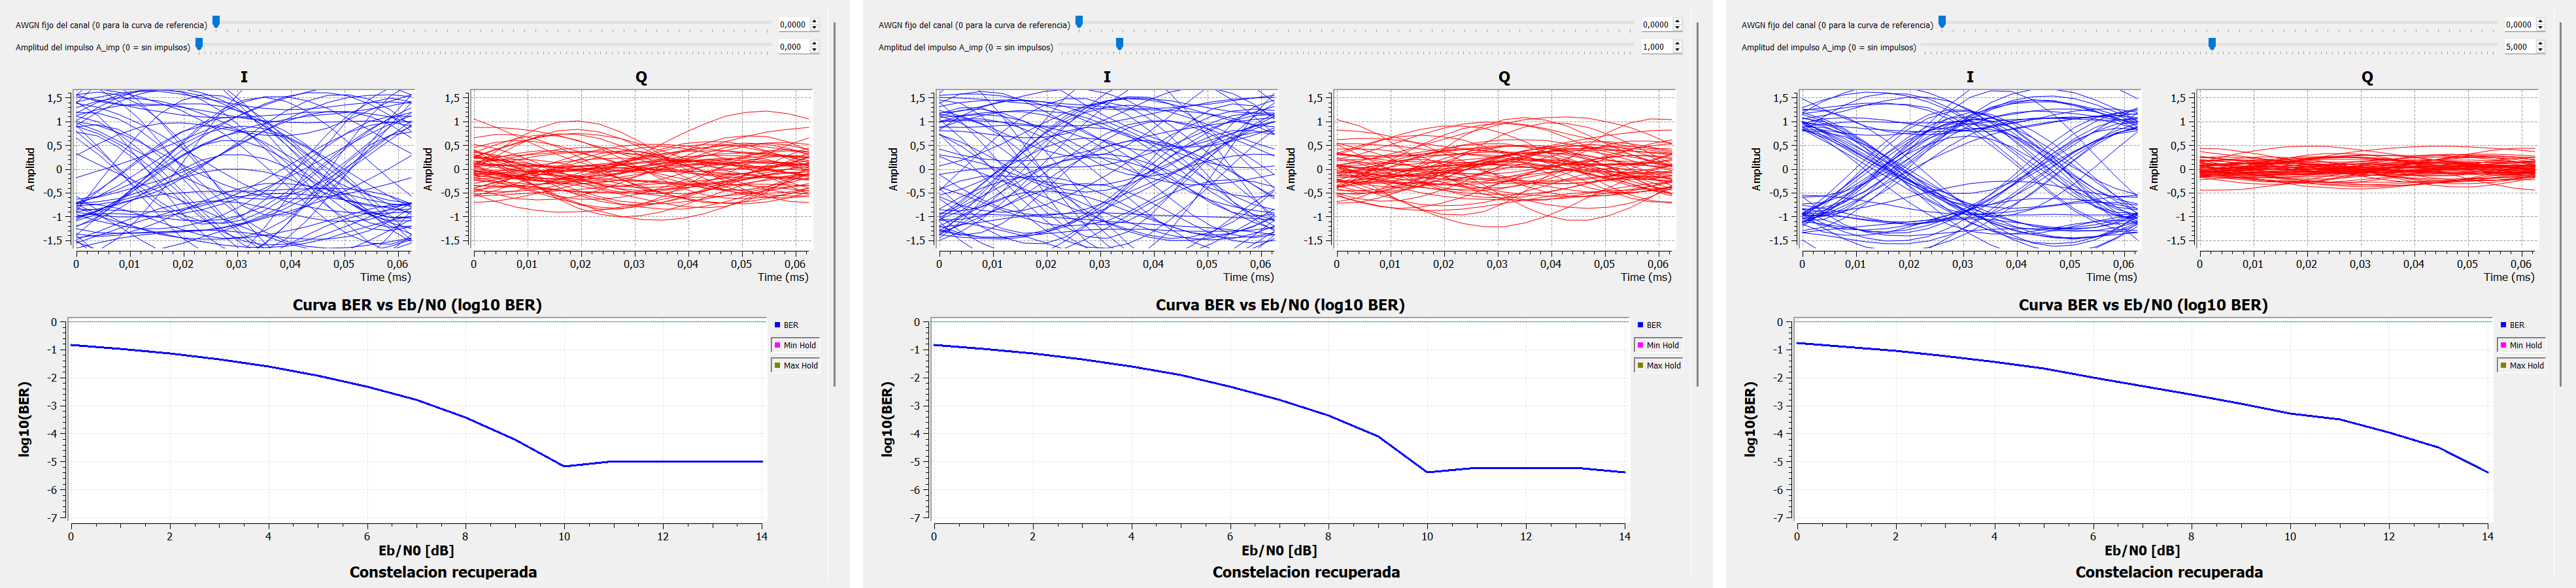
\includegraphics[width=\textwidth]{Figuras/fase4_ventanas.png}
    \caption{Ventanas de los flujogramas de la Fase~4 después de 4 minutos de barrido: sin impulsos (izquierda), $A_{imp}=1$ (centro) y $A_{imp}=5$ (derecha).}
    \label{fig:ventanas}
\end{figure*}
La Fig.~\ref{fig:ventanas} muestra las ventanas de GNU Radio con las que se obtuvieron las curvas de la Fig.~\ref{fig:ber}. El eje vertical es $\log_{10}(\mathrm{BER})$. El ojo de la parte superior corresponde al nivel de ruido del punto del barrido que estaba activo en el momento de la captura, por eso aparece cerrado. En las curvas sin impulsos y con $A_{imp}=1$, el tramo plano a la derecha corresponde a puntos sin errores, que la gráfica dibuja con la cota $3/N$. La curva con $A_{imp}=5$ queda por encima en todo el rango y desciende de forma gradual.

\subsection{Flujograma de medición BER (Fase 4)}
\label{app:fase4}
\begin{figure*}[t]
    \centering
    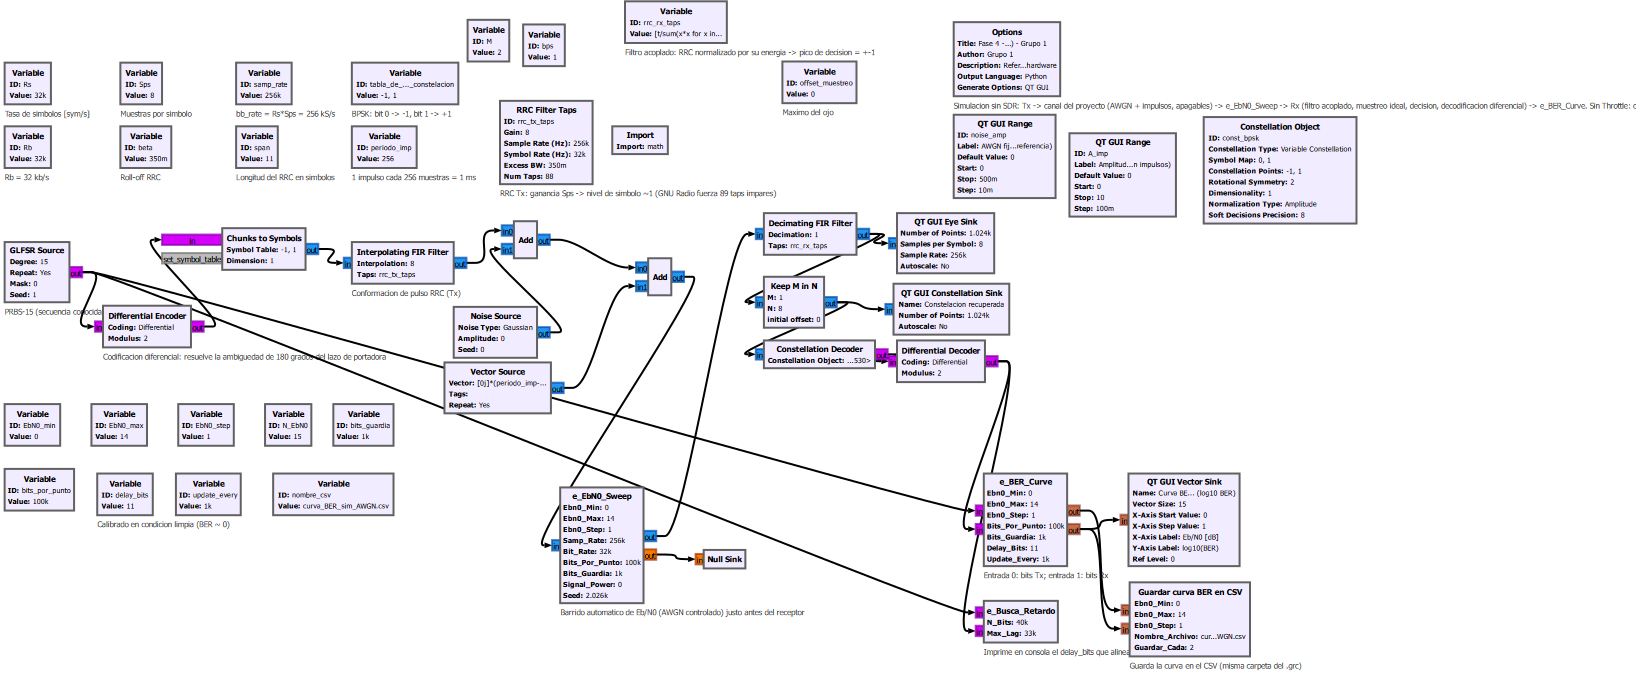
\includegraphics[width=\textwidth]{Figuras/flujograma_fase4.png}
    \caption{Flujograma de medición BER: transmisor con codificación diferencial, canal (AWGN e impulsos), \texttt{e\_EbN0\_Sweep} justo antes del filtro acoplado, receptor (filtro acoplado, muestreo, decisión y decodificación diferencial), \texttt{e\_BER\_Curve} con los bits de la fuente PRBS y los bits recuperados, \texttt{e\_Busca\_Retardo} y el bloque que guarda el CSV.}
    \label{fig:fase4}
\end{figure*}
La Fig.~\ref{fig:fase4} muestra dónde se integró el instrumento. El barrido de ruido se aplica a la señal compleja a 256~kS/s que entra al receptor, y la comparación de bits se hace después de la decodificación diferencial, con la referencia tomada antes del codificador.

\subsection{Evidencias de la práctica de laboratorio}
\label{app:lab}
\begin{figure}[H]
    \centering
    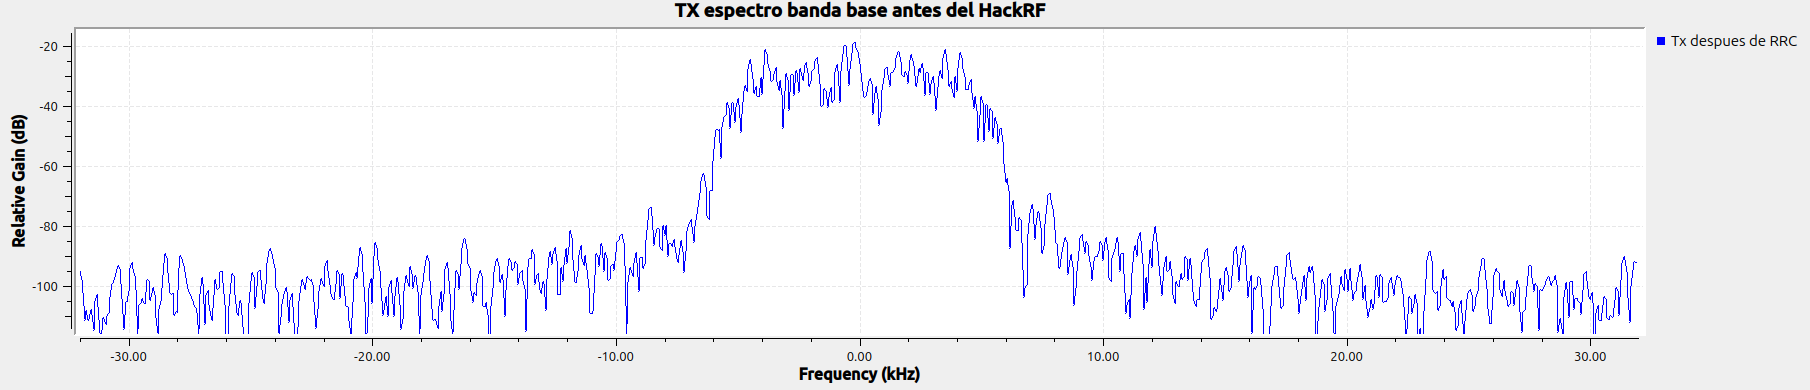
\includegraphics[width=\linewidth]{Figuras/lab_tx_espectro.png}
    \caption{Transmisor HackRF de la práctica de laboratorio: espectro en banda base antes del radio (16-QAM con RRC de roll-off 0.5).}
    \label{fig:lab_tx}
\end{figure}
La Fig.~\ref{fig:lab_tx} muestra el espectro en banda base del transmisor de la práctica. Ocupa unos $\pm6$~kHz, que coinciden con $(1+0.5)\times8$~kHz, y los lóbulos laterales quedan unos 60~dB por debajo.

\begin{figure*}[!t]
    \centering
    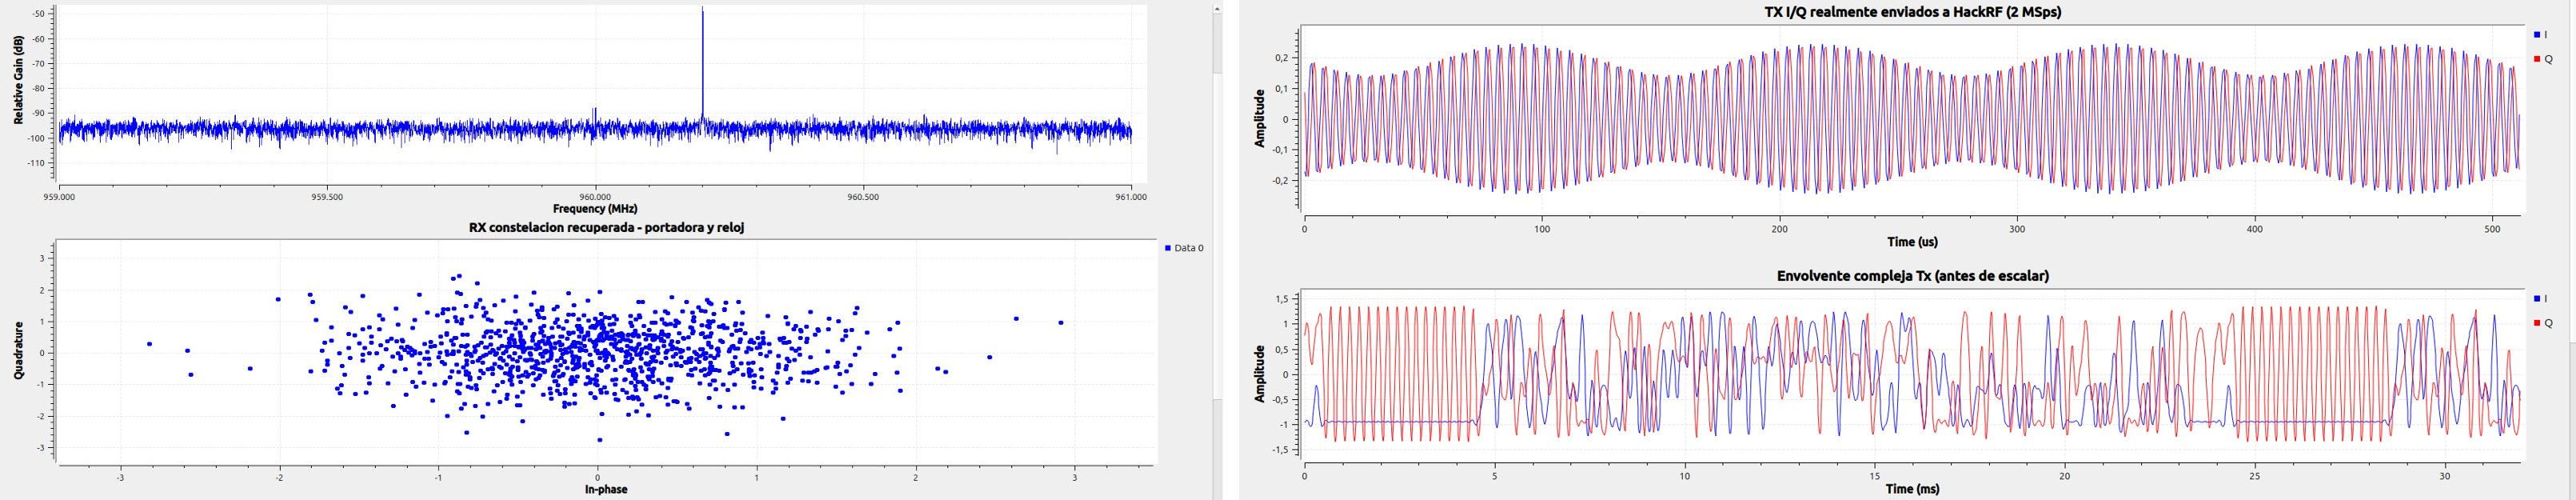
\includegraphics[width=\textwidth]{Figuras/lab_extra.jpg}
    \caption{Práctica de laboratorio. Izquierda: receptor con el transmisor detenido (10:30). Derecha: muestras I/Q enviadas al HackRF (2~MS/s) y envolvente compleja antes de escalar.}
    \label{fig:lab_extra}
\end{figure*}
En la Fig.~\ref{fig:lab_extra}, a la izquierda, sin transmisión el espectro solo conserva la componente de continua del receptor en 960.2~MHz y la constelación se convierte en una nube de ruido centrada en el origen; la amplitud de la salida del filtro baja de $\approx0.1$ a $\approx0.004$. A la derecha, las muestras I/Q realmente enviadas al radio tienen un pico cercano a 0.2, por debajo del límite de 1 del conversor, porque la amplitud digital se fijó en 0.15. Así el transmisor trabaja sin saturar y la potencia se ajusta con la ganancia de RF.

\clearpage


\begin{thebibliography}{9}

\bibitem{blackard1993} K. L. Blackard, T. S. Rappaport y C. W. Bostian, ``Measurements and models of radio frequency impulsive noise for indoor wireless communications,'' \emph{IEEE J. Sel. Areas Commun.}, vol. 11, no. 7, pp. 991--1001, 1993.

\bibitem{middleton1977} D. Middleton, ``Statistical-physical models of electromagnetic interference,'' \emph{IEEE Trans. Electromagn. Compat.}, vol. EMC-19, no. 3, pp. 106--127, 1977.

\bibitem{zhan2022} M. Zhan, Z. Pang, D. Dzung, K. Yu y M. Xiao, ``Short-packet interleaver against impulse interference in practical industrial environments,'' arXiv:2203.00770, 2022.

\bibitem{proakis2008} J. G. Proakis y M. Salehi, \emph{Digital Communications}, 5.ª ed. Nueva York, NY, EE.\,UU.: McGraw-Hill, 2008.

\bibitem{ortega2019} H. Ortega Boada y Ó. M. Reyes Torres, \emph{Comunicaciones digitales basadas en radio definida por software}, Editorial UIS, 2019.

\bibitem{hackrf} Great Scott Gadgets, ``HackRF One documentation.'' [En línea]. Disponible: \url{https://hackrf.readthedocs.io/en/stable/hackrf_one.html}

\bibitem{uhd} Ettus Research, ``UHD manual.'' [En línea]. Disponible: \url{https://files.ettus.com/manual/}

\bibitem{gnuradio} GNU Radio Project, ``GNU Radio.'' [En línea]. Disponible: \url{https://www.gnuradio.org}

\end{thebibliography}
 




% Insert bibliography from .bib
%\bibliographystyle{ieeetr}
%\bibliography{references}

% Warning to check in detail for any remanent template text.
\vspace{12pt}

\end{document}
